% ISEG MASTER DISSERTATION
% MASTER'S IN MATHEMATICAL FINANCE
% AUTHOR: Petr Terletskiy
% SUPERVISOR: Prof. João Afonso Bastos
%
% Based on the ISEG template by Costa (2017),
% adapted by Domingos Guerreiro Seward and Luís F. Costa (2018).
%
% NOTE: Compile with pdfLaTeX (or XeLaTeX if fontspec is used)
%
% =============================================
% Preamble
% =============================================

\documentclass[12pt,a4paper,oneside]{article}

% Font
\usepackage{times}
\usepackage[T1]{fontenc}
\usepackage[utf8]{inputenc}

% Language
\usepackage[english]{babel}

% Appendix
\usepackage[toc,page]{appendix}

\makeatletter
\def\@biblabel#1{\hspace*{-\labelsep}}
\makeatother

% Bibliography
\usepackage[authoryear,round]{natbib}
\bibliographystyle{plainnat}

% Margins (3cm all sides per ISEG guidelines)
\usepackage[top=3cm, bottom=3cm, left=2.9cm, right=2.9cm]{geometry}

% Change margins command
\def\changemargin#1#2{\list{}{\rightmargin#2\leftmargin#1}\item[]}
\let\endchangemargin=\endlist

% Paragraph indentation
\usepackage{indentfirst}

% 1.5 line spacing
\usepackage{setspace}
\onehalfspacing

% Paragraph spacing
\parskip=6pt

% Headers and footers
\usepackage{fancyhdr}
\pagestyle{fancy}
\fancyhf{}
\lhead{\footnotesize \textsc{Petr Terletskiy}}
\rhead{\footnotesize\textsc{BTC Direction Prediction Using KANs}}
\cfoot{\thepage}

% Section formatting
\usepackage{titlesec}
\titleformat{\chapter}[display]
  {\scshape\center}
  {}
  {0pt}
  {\thechapter.\ }
\usepackage{etoolbox}
\makeatletter
\patchcmd{\chapter}{\if@openright\cleardoublepage\else\clearpage\fi}{}{}{}
\makeatother
\titleformat{\section}
  {\scshape\center}{\thesection}{1em}{}
\titleformat{\subsection}
  {\itshape\center}{\thesubsection}{1em}{}
\titleformat{\subsubsection}
  {\itshape\center}{\thesubsubsection}{1em}{}

% Hyperlinks
\usepackage{hyperref}
\hypersetup{
    colorlinks=true,
    linkcolor=black,
    citecolor=black,
    urlcolor=blue
}

% Table of contents
\usepackage{tocloft}
\setlength{\cftbeforetoctitleskip}{0pt}
\setlength{\cftbeforeloftitleskip}{0pt}
\setlength{\cftbeforelottitleskip}{0pt}

% Tables
\renewcommand*\thetable{\Roman{table}}
\addto\captionsenglish{\renewcommand{\tablename}{\textsc{Table}}}
\addto\captionsenglish{\renewcommand{\figurename}{\textsc{Figure}}}

\usepackage{lipsum}
\usepackage{booktabs}
\usepackage{adjustbox}
\setlength\heavyrulewidth{0.3ex}
\usepackage{tabularx}
\usepackage{array}
\usepackage{threeparttable}
\usepackage{multirow}
\usepackage{longtable}

% Quotes
\usepackage{csquotes}

% Mathematics
\usepackage{amsmath}
\usepackage{amsfonts}
\usepackage{amssymb}
\usepackage{bm}

% Graphics
\usepackage{graphicx}
\graphicspath{{figures/}}
\usepackage{float}
\usepackage{subcaption}
\usepackage{chngcntr}
\counterwithin{figure}{section}
\counterwithin{table}{section}
\usepackage{tikz}
\usetikzlibrary{arrows.meta, positioning}

% Code listings (for algorithm pseudocode)
\usepackage{algorithm}
\usepackage{algpseudocode}

% Glossary / Acronyms
\usepackage[automake]{glossaries}
\makeglossaries

% ── Acronyms ──────────────────────────────────────────────────────────
% AFML \& Methodology
\newacronym{afml}{AFML}{Advances in Financial Machine Learning}
\newacronym{tbl}{TBL}{Triple Barrier Labeling}
\newacronym{cusum}{CUSUM}{Cumulative Sum}
\newacronym{ffd}{FFD}{Fixed-width Window Fractional Differentiation}
\newacronym{cpcv}{CPCV}{Combinatorial Purged Cross-Validation}
\newacronym{dsr}{DSR}{Deflated Sharpe Ratio}
\newacronym{pbo}{PBO}{Probability of Backtest Overfitting}
\newacronym{mda}{MDA}{Mean Decrease Accuracy}

% Models
\newacronym{kan}{KAN}{Kolmogorov-Arnold Network}
\newacronym{lstm}{LSTM}{Long Short-Term Memory}
\newacronym{rf}{RF}{Random Forest}
\newacronym{xgb}{XGBoost}{Extreme Gradient Boosting}
\newacronym{lr}{LR}{Logistic Regression}
\newacronym{ar}{AR}{Autoregressive}
\newacronym{mlp}{MLP}{Multi-Layer Perceptron}

% Technical
\newacronym{btc}{BTC}{Bitcoin}
\newacronym{ohlcv}{OHLCV}{Open-High-Low-Close-Volume}
\newacronym{ta}{TA}{Technical Analysis}
\newacronym{ewma}{EWMA}{Exponentially Weighted Moving Average}
\newacronym{adf}{ADF}{Augmented Dickey-Fuller}
\newacronym{rsi}{RSI}{Relative Strength Index}
\newacronym{macd}{MACD}{Moving Average Convergence Divergence}
\newacronym{atr}{ATR}{Average True Range}
\newacronym{obv}{OBV}{On-Balance Volume}
\newacronym{mfi}{MFI}{Money Flow Index}
\newacronym{cci}{CCI}{Commodity Channel Index}
\newacronym{vix}{VIX}{CBOE Volatility Index}
\newacronym{mvrv}{MVRV}{Market Value to Realized Value}
\newacronym{sadf}{SADF}{Supremum Augmented Dickey-Fuller}

% Financial
\newacronym{mfw}{MFW}{Master's Final Work}
\newacronym{jel}{JEL}{Journal of Economic Literature}
\newacronym{emh}{EMH}{Efficient Market Hypothesis}


% =============================================
% Begin Document
% =============================================

\begin{document}

% ── 1. Cover Page ─────────────────────────────────────────────────────
\begin{titlepage}
    \begin{flushleft}
        \includegraphics[width=5cm]{ISEG_logo.png}
    \end{flushleft}
    
    \vspace{1.5cm}
    
    \begin{center}
        {\Large \textsc{Master}}\\[0.5cm]
        {\Large \textsc{MATHEMATICAL FINANCE}}\\[2cm]
        
        {\Large \textsc{Master's Final Work}}\\[0.5cm]
        {\Large \textsc{PROJECT}}\\[3cm]
        
        {\LARGE \textbf{BITCOIN DIRECTION PREDICTION USING KOLMOGOROV-ARNOLD NETWORKS WITHIN THE AFML FRAMEWORK}}\\[3cm]
        
        {\Large \textsc{Petr Terletskiy}}\\[1.5cm]
                
        \vfill
        
        {\large \textsc{May 2026}}
    \end{center}
\end{titlepage}

% ── 2. Title Page (Inside Cover) ──────────────────────────────────────
\begin{titlepage}
    \begin{flushleft}
        \includegraphics[width=5cm]{ISEG_logo.png}
    \end{flushleft}
    
    \vspace{1.5cm}
    
    \begin{center}
        {\Large \textsc{Master}}\\[0.5cm]
        {\Large \textsc{MATHEMATICAL FINANCE}}\\[1.5cm]
        
        {\Large \textsc{Master's Final Work}}\\[0.5cm]
        {\Large \textsc{PROJECT}}\\[2cm]
        
        {\LARGE \textbf{BITCOIN DIRECTION PREDICTION USING KOLMOGOROV-ARNOLD NETWORKS WITHIN THE AFML FRAMEWORK}}\\[2cm]
        
        {\Large \textsc{Petr Terletskiy}}\\[2cm]
        
        {\large \textsc{Supervision:}}\\[0.2cm]
        {\Large \textsc{Prof. João Afonso Bastos}}\\[2cm]
        
        \vfill
        
        {\large \textsc{May 2026}}
    \end{center}
\end{titlepage}

% ── 3. Blank Page ─────────────────────────────────────────────────────
\newpage
\thispagestyle{empty}
\mbox{}

% ── 4. Dedication ─────────────────────────────────────────────────────
\newpage
\thispagestyle{empty}
\vspace*{\fill}
\begin{flushright}
\textit{%
To my family and God.
}
\end{flushright}

% ── 5. Erratum (commented out unless needed for final post-viva) ──────
%\newpage
%\thispagestyle{plain}
%\addcontentsline{toc}{section}{Erratum}
%\section*{Erratum}

% ── 6. Glossary ───────────────────────────────────────────────────────
\newpage
\thispagestyle{plain}
\addcontentsline{toc}{section}{Glossary}

\setcounter{page}{1}
\pagenumbering{roman}

\glsaddall
\printglossaries


% ── 7. Abstract ───────────────────────────────────────────────────────
\newpage
\thispagestyle{plain}
\addcontentsline{toc}{section}{Abstract, Keywords, and JEL Codes}

\section*{Abstract, Keywords, and \gls{jel} Codes}

% TODO: Write abstract (300 words max).
%
% Topics to cover, mapping the paper_outline narrative:
%   - Frame around Q1 to Q4 / C1 to C4 from the outline.
%   - Headline numbers from the locked run (v6, 5 seeds across all six models,
%     840 prediction entries, 1,168 aligned events, base rate 0.5685):
%       * No model achieves DSR >= 0.95 (top DSR among trained models =
%         0.2470, KAN).
%       * Buy-and-hold posts a higher median Sharpe (2.2722) than every
%         trained model; DSR is not defined for buy-and-hold since it
%         does not enter the Optuna selection pool.
%       * PBO = 0.657 lands in the adversarial regime (23 of 35 IS/OOS
%         partitions); the IS-best is the OOS-loser in nearly two of three
%         partitions. 6 of 7 bootstrap 95\% CIs cross zero; only
%         buy-and-hold's CI (1.8903, 2.4685) stays strictly positive.
%         The previous run's KAN strict-positive CI (0.0971, 1.2413)
%         does NOT reproduce under uniform 5-seed evaluation; KAN's CI
%         is now (-0.4677, 1.1607). Leave-one-out PBO shows Random
%         Forest is the PBO-anchor (Delta +0.000), while every other
%         model's exclusion reduces PBO; Logistic Regression is the
%         largest destabiliser (Delta -0.286 to 0.371).
%       * DeLong: 2 of 15 pairwise AUC tests reach alpha=0.05 (AR
%         Logistic vs XGBoost p=0.0427, Random Forest vs XGBoost
%         p=0.0318), both with XGBoost as the lower-AUC half. The
%         first locked configuration with any DeLong-significant pair.
%       * Symbolic extraction succeeds: 100\% symbolification rate (15
%         of 15 edges, no skips), three surviving features
%         (eth\_btc\_ratio, log\_returns\_lag6, natgas\_ret\_30),
%         post-symbolic accuracy 51.85\% (a 5.18 pp gain over
%         pre-symbolic 46.67\%, but both numbers sit at or below the 50\%
%         baseline). The symbolic-extraction outputs are identical to
%         the previous 3-seed run (PyKAN retrained with fixed seed on
%         same training fold). The Phase-1 dynamic gate (max(0.53,
%         base\_rate + 0.01) = 0.5693) fails at val\_acc 0.4815 and the
%         pre-prune gate also fails; the locked-run PyKAN model has not
%         extracted directional signal on the deployment fold. The
%         formula uses six clean primitives (sin, cos, tanh, x\^2, x\^3,
%         x\^4); the previous configuration's Abs(.) non-
%         differentiability flag is resolved and all surviving features
%         have finite gradients everywhere. A lag feature
%         survives extraction for the second consecutive locked
%         configuration (log\_returns\_lag1 -> log\_returns\_lag6).
%   - Position the symbolic contribution as the first closed-form
%     classification formula extracted from a CPCV-trained KAN under
%     the full AFML evaluation.
This dissertation evaluates whether Kolmogorov-Arnold Networks can predict Bitcoin daily price direction and extract interpretable symbolic formulas, benchmarked against five models within López de Prado's Advances in Financial Machine Learning framework. Using Combinatorial Purged Cross-Validation with the Deflated Sharpe Ratio and Probability of Backtest Overfitting, the study finds that no model achieves statistically significant predictive performance, consistent with market efficiency. The core contribution is KAN symbolic expression extraction, deriving closed-form decision functions from the trained network.

\vspace{1em}

\textsc{Keywords}: Bitcoin; Kolmogorov-Arnold Networks; Symbolic Extraction; Triple Barrier Labeling; Combinatorial Purged Cross-Validation; Financial Machine Learning.

\vspace{1em}

\textsc{\gls{jel} Codes}: C45; C53; C58; G11; G17.


% ── 8. Table of Contents ──────────────────────────────────────────────
\newpage
\thispagestyle{plain}
\addcontentsline{toc}{section}{Table of Contents}
\renewcommand*\contentsname{\hfill\normalfont\scshape\normalsize Table of Contents \hfill}
\tableofcontents

% ── 9. List of Figures ────────────────────────────────────────────────
\newpage
\thispagestyle{plain}
\addcontentsline{toc}{section}{List of Figures}
\renewcommand*\listfigurename{\hfill\normalfont\scshape\normalsize List of Figures \hfill}
\listoffigures

% ── 10. List of Tables ────────────────────────────────────────────────
\newpage
\thispagestyle{plain}
\addcontentsline{toc}{section}{List of Tables}
\renewcommand*\listtablename{\hfill\normalfont\scshape\normalsize List of Tables \hfill}
\listoftables

% ── 11. Preface (optional) ────────────────────────────────────────────
%\newpage
%\thispagestyle{plain}
%\addcontentsline{toc}{section}{Preface}
%\section*{Preface}


% ── 12. Acknowledgements ──────────────────────────────────────────────
\newpage
\thispagestyle{plain}
\addcontentsline{toc}{section}{Acknowledgements}
\section*{Acknowledgements}

% TODO: Write acknowledgements.
First, I wish to thank Professor João Afonso Bastos for his encouragement and guidance. I am also thankful to my family for their patience and support while I pursued this project.


% =============================================
% TEXTUAL PART BEGINS
% =============================================
\newpage
\thispagestyle{plain}

\setcounter{page}{1}
\pagenumbering{arabic}

\begin{center}
\textsc{BITCOIN DIRECTION PREDICTION USING KOLMOGOROV-ARNOLD NETWORKS WITHIN THE AFML FRAMEWORK BY PETR TERLETSKIY}\\
\end{center}


% ==================================================================
% CHAPTER 1: INTRODUCTION
% ==================================================================
\section{Introduction}\label{sec:introduction}

This thesis applies a Kolmogorov-Arnold Network (KAN) to Bitcoin (BTC) price direction prediction under the full Advances in Financial Machine Learning (AFML) framework \citep{lopez_de_prado_2018}. The KAN is benchmarked against five baselines drawn from the econometric, linear, ensemble, and recurrent neural families on identical cross-validation splits, features, and sample weights. The novel deliverable is a closed-form symbolic decision function for the probability of an upward move ($P(\text{Up})$), extracted from the trained KAN.

The headline finding is negative on the predictive side and positive on the interpretive side. Under leakage-free evaluation with multiple-testing correction, no trained model in the benchmark demonstrates a statistically significant predictive edge. The deflated Sharpe ratio of the best trained model sits well below the conventional significance threshold, and the probability of backtest overfitting lands in the adversarial regime, meaning the in-sample best model is the out-of-sample loser more often than not. A naive buy-and-hold strategy on the same data outperforms every trained model on median Sharpe, at the cost of carrying the full BTC drawdown profile. The symbolic-extraction pipeline, by contrast, succeeds on its own terms. Every spline edge of the trained KAN finds a clean symbolic match, and the resulting closed-form decision function is humanly readable. Interpretability turns out to be a separable contribution from predictive accuracy, and one that does not need to wait for predictive significance to be valuable.


\subsection{Research Context and Motivation}\label{subsec:context}

% Why BTC

Bitcoin (BTC) was presented to the world on October 31, 2008 by Satoshi Nakamoto. Since its first transaction on January 12, 2009, BTC has produced one of the highest cumulative returns of any major asset, and it gave birth to the cryptocurrency asset class. It is today the largest cryptocurrency by market capitalization. Unlike traditional asset classes, BTC trades 365 days a year, 24/7 on a transparent and publicly auditable blockchain, exposing on-chain activity that has no equivalent in equity or fixed-income markets.

% Why KANs

Machine Learning (ML) adoption in financial markets has grown exponentially. Unlike classical econometric methods that impose functional forms a priori, ML models are capable of inferring structure directly from the data, which suits the non-linear behaviour of asset returns. However, most ML models, and Neural Networks in particular, operate as black boxes whose internal logic cannot be directly interpreted. Liu et al.\ \citeyearpar{liu_kan_2024} propose KANs, a Multi-Layer Perceptron (MLP) alternative whose edges carry learnable B-splines that can be distilled into closed-form symbolic functions, offering interpretability that conventional Deep Learning (DL) architectures do not provide. To the author's knowledge, no prior work applies KANs to BTC price direction prediction or extracts symbolic formulas from a classification KAN under the AFML framework \citep{lopez_de_prado_2018}. This gap defines the four research questions of this thesis.


\subsection{Problems and Research Questions}\label{subsec:objectives}

% Q1
\textbf{Q1.} Many recent BTC ML studies report daily-direction accuracies of 85 to 95 percent \citep{omole_enke_2024}, but the figures rest on pipelines with fixed-horizon labels, overlapping label spans, and train-test splits that never purge concurrent observations. Under those conditions, training labels carry information about test-period prices and the reported accuracies may be inflated by an unknown margin. This thesis asks whether BTC daily direction remains predictable once labels and features stop leaking the future and overlapping observations are properly weighted. The answer is tested through three corrections on a six-model cross-section: the Deflated Sharpe Ratio (DSR), the Probability of Backtest Overfitting (PBO), and pairwise DeLong Area Under the Curve (AUC) comparisons.

% Q2
\textbf{Q2.} Most cryptocurrency ML studies rely on one or two feature families, typically technical indicators or price histories \citep{bourday_crypto_dl_2024}, and there is no consensus on whether macroeconomic, crypto-macro, or on-chain features add information beyond price-derived inputs. This thesis asks which families carry signal under a leakage-free evaluation, and whether on-chain features could deliver additional alpha over price-derived inputs. Per-family selection frequencies recorded by multi-model permutation importance across the 28 Combinatorial Purged Cross-Validation (CPCV) folds provide the answer.

% Q3
\textbf{Q3.} KANs have been applied to VIX forecasting \citep{cho_lee_kim_2025}, stock prediction \citep{oad_kasper_2025}, and cryptocurrency regression \citep{gao_decokan_2025}, but never to BTC direction classification. Their position relative to econometric, linear, tree-based, and deep-learning baselines on a uniform protocol is therefore unknown. This thesis asks where the KAN sits in a six-model cross-section evaluated under identical CPCV splits, features, sample weights, and metrics, with Autoregressive (AR) Logistic, Logistic Regression, Random Forest, Extreme Gradient Boosting (XGBoost), and Long Short-Term Memory (LSTM) as the baselines.

% Q4
\textbf{Q4.} Existing KAN symbolic-extraction work in finance targets regression problems on relatively predictable series \citep{cho_lee_kim_2025, oad_kasper_2025, gao_decokan_2025}. To the author's knowledge, no published work has extracted a closed-form classification formula from a CPCV-trained KAN in a weak-signal regime. This thesis asks whether a human-readable expression for $P(\text{Up})$ can be extracted from a CPCV-trained KAN while preserving most of its predictive accuracy.


\subsection{Contributions}\label{subsec:contributions}

% C1
\textbf{C1.} This thesis applies the complete AFML stack to BTC direction prediction: Cumulative Sum (CUSUM) event sampling, triple-barrier labeling (TBL), sample weighting, fractional differencing, CPCV with purging and embargo, and the DSR, PBO, and DeLong AUC corrections. The pipeline implements every leakage and multiple-testing safeguard the framework prescribes in a single reproducible workflow.

% C2
\textbf{C2.} This thesis assembles a 73-feature universe spanning four families: 25 technical, 9 statistical, 29 external (macroeconomic, crypto-macro, and on-chain), and 10 autoregressive lag features. All 73 features compete in multi-model permutation importance selection across the 28 CPCV folds, with no family privileged a priori.

% C3
\textbf{C3.} This thesis benchmarks the KAN against the five baselines under identical CPCV splits, features, sample weights, and metrics. Pairwise DeLong AUC tests identify which differences across the six-model cross-section reach statistical significance.

% C4
\textbf{C4.} This thesis extracts a human-readable mathematical expression for $P(\text{Up})$ from the trained KAN via PyKAN's prune-and-symbolify pipeline. To the author's knowledge, this is the first closed-form classification formula derived from a CPCV-trained KAN in a weak-signal regime, and the primary novel contribution of this work.


\subsection{Document Structure}\label{subsec:structure}

Section 2 reviews the literature on KANs, ML for BTC prediction, and the AFML methodology. Section 3 details the data and the full empirical pipeline. Section 4 reports the results, Section 5 discusses them, Section 6 concludes the thesis and outlines directions for future work.


% ==================================================================
% CHAPTER 2: LITERATURE REVIEW
% ==================================================================
\newpage
\section{Literature Review}\label{sec:literature}

% Cochrane: position against the 2 to 3 closest papers per stream.
% Three streams: KANs, BTC ML prediction, AFML methodology.
% Each stream ends with a gap statement.
%
% Placement notes from the outline:
%   - HARd to Beat (Chassot \& Audrino 2026) goes in 2.3.9 (AFML),
%     NOT in BTC ML. The paper is methodological; its claim
%     ("fitting scheme matters more than model choice") supports
%     this thesis's DSR=0 narrative directly.
%   - Kolmogorov-Arnold theorem and splines go in 2.1 only. NOT in
%     Introduction (no math before main result). NOT in Methodology
%     (Methodology assumes the reader has read 2.1).


\subsection{Kolmogorov-Arnold Networks}\label{subsec:lit_kan}

\subsubsection{Mathematical foundation}\label{subsubsec:kan_math}

The Kolmogorov-Arnold representation theorem decomposes any continuous multivariate function into a finite sum of continuous univariate functions. The result settled Hilbert's thirteenth problem, which asked whether every continuous function of three variables could be written as a superposition of continuous functions of at most two variables. Hilbert thought not. He was wrong. \citet{arnold_1958} confirmed the conjecture for three variables, and \citet{kolmogorov_1957} established the general result, proving that any continuous function $f : [0,1]^n \to \mathbb{R}$ admits the representation
\begin{equation}
f(x_1, \ldots, x_n) = \sum_{q=1}^{2n+1} \Phi_q \! \left( \sum_{p=1}^{n} \varphi_{q,p}(x_p) \right),
\label{eq:kst}
\end{equation}
where $\varphi_{q,p}$ and $\Phi_q$ are continuous univariate functions. Multivariate continuous functions can always be written using only sums and univariate functions of single inputs, which makes addition the only genuinely multivariate operation.

The catch is that the inner functions $\varphi_{q,p}$ in Kolmogorov's construction can be highly non-smooth and even fractal, and no universal inner family is compatible with $C^1$ regularity \citep{liu_kan_2024}. For decades the theorem was therefore considered theoretically sound but practically useless for neural-network design. \citet{liu_kan_2024} reopened the question on two fronts. They parameterised each univariate function as a learnable B-spline rather than insisting on the pathological inner functions of the original existence proof, and they generalised the architecture beyond the two-layer, $2n+1$-width form to arbitrary widths and depths. The justification is empirical rather than mathematical: most functions of practical interest are smooth and have sparse compositional structure, so smooth splines can approximate the Kolmogorov-Arnold decomposition even if they cannot realise it exactly without giving up smoothness. Under these relaxations the authors prove an approximation bound of order $\mathcal{O}(G^{-k-1+m})$ in the $C^m$-norm for $k$-th order B-splines on a grid of size $G$, a rate independent of the input dimension $n$ that therefore avoids the curse of dimensionality.


\subsubsection{How KANs work}\label{subsubsec:kan_arch}

The architectural move that makes KANs interpretable is small but consequential. Where an MLP places fixed activation functions on nodes and learns scalar weights on edges, a KAN places learnable activation functions on edges and lets the nodes do nothing but sum \citep{liu_kan_2024}. Each edge parameterises its activation as a B-spline
\begin{equation}
g(x) = \sum_{k=0}^{K} a_k B_k(x),
\label{eq:kan_edge}
\end{equation}
of order $K$ over $G$ grid intervals, with coefficients $a_k$ trained alongside the rest of the network. A KAN is then specified by a width vector $[n_{\text{input}}, n_{\text{hidden}}, n_{\text{output}}]$ analogous to an MLP, except that every directed edge between layers carries one trainable univariate spline rather than a single scalar weight.

Training follows a two-phase schedule. Adam runs first to push the loss into a good basin and escape shallow local minima, and L-BFGS finishes the optimisation by exploiting second-order curvature once Adam has positioned the model correctly. The loss carries two sparsity penalties on top of the prediction term: an $L_1$ term on edge activations that drives small-magnitude splines toward zero, and an entropy term that concentrates importance on a few edges rather than spreading it across many. The two penalties together allow a trained KAN to be pruned cleanly without losing predictive performance, and they make the surviving edges amenable to symbolic replacement.

The property exploited in this thesis lies in what happens after training. Each retained edge's spline is a numerically defined univariate function, and PyKAN provides a library of symbolic candidates ($\sin$, $\cos$, $\exp$, $\tanh$, $x^2$, and others) that can be matched against the learned shape \citep{liu_kan_2024}. Once every retained edge has been replaced by its best symbolic match, the network collapses to a closed-form expression in the input features. This final step is unique to KANs: no other neural family decomposes cleanly into univariate functions whose shapes can be read off, named, and substituted.


\subsubsection{KAN variants}\label{subsubsec:kan_variants}

A growing ecosystem of KAN variants has emerged since the original 2024 release, ranging from polynomial-basis substitutions (ChebyKAN, Jacobi KANs), wavelet-basis variants (Wav-KAN), Gaussian RBF substitutes for splines (FastKAN), and architectural extensions for sequential data. \citet{yamak_et_al_2025} synthesise roughly forty of these under a single survey, sparing this thesis the need to cite each individually, and note that symbolic distillation specifically applied to financial time series remains underexplored. Two variants from the survey are worth singling out because they are directly relevant to the design choices made here.

First, KAN 2.0 \citep{liu_kan2_2024} introduces multiplication nodes alongside the original addition nodes, allowing the architecture to discover multiplicative interactions between features (for example, an interaction term like $\text{RSI} \times \text{Stoch\_K}$) without forcing the network to recover them through a log-exp decomposition. The same train-prune-symbolify pipeline applies unchanged, which makes KAN 2.0 a natural next step for a follow-up study that extends the symbolic distillation reported here to interaction-rich feature sets. KAN 2.0 is cited as a future-work direction rather than implemented in the main results.

Second, the Temporal Kolmogorov-Arnold Network (TKAN) of \citet{genet_inzirillo_2024} replaces the dense linear gates of an LSTM cell with KAN-parameterised gates, giving the architecture explicit memory at the cost of breaking the static feedforward structure that PyKAN's symbolic-extraction pipeline depends on. TKAN is therefore representative of the architectural-variant literature this thesis chose not to pursue: sequence-aware extensions are powerful for multi-step forecasting but incompatible with closed-form formula extraction.


\subsubsection{KANs in finance and the gap}\label{subsubsec:kan_finance}

Three recent applications of KANs to financial time series bracket what this thesis does and does not do.

\citet{cho_lee_kim_2025} apply KANs to forecasting the CBOE Volatility Index (VIX) and, in doing so, introduce the four-step symbolic-extraction pipeline that this thesis adapts with minimal modification. The pipeline trains a small KAN with $L_1$ and entropy regularisation, prunes low-importance edges and nodes once the validation loss stops improving, replaces each surviving spline with the best-matching symbolic function from a candidate library, and fine-tunes the affine parameters introduced during symbolification. The extracted formulas recover well-known stylised facts of the VIX with explicit coefficients. The pipeline is the direct methodological ancestor of what this thesis applies to BTC daily direction, with one important caveat: the VIX is mean-reverting and structurally predictable, while BTC daily direction is binary classification in a weak-signal regime, which makes the same pipeline substantially harder to satisfy.

\citet{oad_kasper_2025} are the closest related work on the KAN-plus-finance-plus-interpretability triangle. Their KASPER framework stacks two KAN layers, the first performing soft regime detection via a Gumbel-Softmax classifier with orthogonality and contrastive regularisation, and the second performing regime-conditioned spline forecasting. They report $R^2 = 0.89$ and a Sharpe ratio of 12.02 on Yahoo Finance stock data, with interpretability achieved through Monte Carlo Shapley rules rather than direct symbolic formula extraction. The architectural distance to this thesis is real: KASPER targets stock-price regression with a regime-detection layer, derives interpretability from Shapley attributions rather than closed-form expressions, and is evaluated under conventional walk-forward splits without an AFML correction layer.

\citet{gao_decokan_2025} are the closest related work on the asset-class axis. DecoKAN combines a multi-level discrete wavelet transform with KAN-based temporal and feature mixers, separating low-frequency macro trends from high-frequency shocks before the KAN mixers handle the nonlinear interactions inside each branch. The paper extracts closed-form expressions for the detail-branch dynamics with $R^2 > 0.99$ on Bitcoin, Ethereum, and Monero daily series. The methodological gap from this thesis is large despite the shared asset class: DecoKAN targets multivariate price-level regression at multiple forecasting horizons, splits the data chronologically without purging or embargo, and reports no DSR, PBO, or related multiple-testing correction.

Three intersecting gaps emerge, and this thesis addresses all three at once. No prior work applies KANs to BTC price direction prediction, since the existing KAN-in-finance literature targets regression problems on the VIX, stock prices, or cryptocurrency price levels. No prior work extracts symbolic formulas from a classification KAN, since the two precedents that distil cleanly (\citet{cho_lee_kim_2025} on VIX, \citet{gao_decokan_2025} on crypto price levels) are both regression on more structurally predictable targets. And no prior work combines KAN symbolic extraction with the AFML framework, since every KAN-in-finance application surveyed above evaluates under conventional chronological splits without purging, embargo, multiple-testing correction, or backtest-overfitting checks. The intersection of all three is the empirical contribution of this thesis.


\subsection{Bitcoin Price Prediction with Machine Learning}\label{subsec:lit_btc}

\subsubsection{Technical analysis and ML for BTC}\label{subsubsec:btc_ta}

\citet{mate_confluence_2024} provide the most directly relevant precedent for the technical-indicator portion of this thesis's feature set. They train four machine-learning models (ANN, CNN-LSTM, SVM, and Random Forest) on 27 technical indicators to classify BTC daily direction, and report classification accuracies of 81\%, 80\%, 82\%, and 81\% respectively. Two of their findings carry directly into the design choices made here. First, the Price Rate of Change (ROC) emerges among the top feature-importance contributors in their analysis, alongside the Stochastic Oscillator components (\%K, \%D) and the Williams Percent Range (\%R), which justifies the inclusion of \texttt{roc\_14} in this thesis's 25-indicator technical feature set. Second, the four-model comparison shows that multi-indicator strategies consistently outperform single-indicator rules, which justifies engineering an indicator universe rather than committing to one canonical signal.

The methodological limitations are instructive: the paper uses standard train-test splits with fixed-horizon labels, no purging or embargo, and equal sample weights, leaving the 80-to-82-percent accuracies attractive on paper but probably inflated under leakage-free re-evaluation. Section~\ref{subsubsec:btc_weaknesses} returns to this critique at the literature level.


\subsubsection{Deep learning for BTC direction}\label{subsubsec:btc_dl}

\citet{omole_enke_2024} target the same problem as this thesis: predicting the daily direction of BTC with a deep-learning classifier. They compare CNN-LSTM, LSTNet, and TCN architectures on a feature set of on-chain blockchain indicators, and use three feature-selection algorithms (Boruta, genetic algorithm, and LightGBM) to address the curse of dimensionality. Their best configuration, Boruta combined with CNN-LSTM, reaches 82.44\% test accuracy on a fixed-horizon binary label, and backtested trading on these predictions reports annualised returns in the thousands of percent.

The methodological gap from this thesis is the cleanest illustration of why headline accuracies in the BTC-ML literature need re-evaluation under leakage-free conditions. \citet{omole_enke_2024} use fixed-horizon labels with no CUSUM event filtering, evaluate on a chronological split without purging or embargo, and weight all observations equally. The 82\% headline accuracy and the four-digit backtest returns are therefore upper bounds on what the same architecture would produce under an AFML evaluation. Section~\ref{subsubsec:btc_weaknesses} extends this critique to the literature as a whole.


\subsubsection{Broader crypto-DL landscape and conservative prediction}\label{subsubsec:btc_dl_landscape}

Beyond the closely related work just discussed, the broader crypto deep-learning landscape contains dozens of further studies surveyed in recent reviews. \citet{wu_crypto_dl_review_2024} compare seven architectures (RNN, LSTM, bidirectional LSTM, GRU, 1D-CNN, TCN, and Transformer) on Bitcoin, Ethereum, Litecoin, and Ripple across pre-COVID and COVID windows, and \citet{bourday_crypto_dl_2024} survey hybrid Transformer-plus-ML approaches with similar coverage. Both reviews document the same recurring methodological issues: small datasets relative to model capacity, overfitting masked by reporting train-set rather than out-of-sample metrics, absence of transaction costs or slippage in backtest evaluations, no risk-adjusted performance metrics such as the Sharpe ratio or maximum drawdown, and inconsistent evaluation protocols that make cross-study comparison difficult. These issues are precisely what the AFML correction layer is designed to address, and they are the reason this thesis treats the 85 to 95 percent accuracy band cited in Section~\ref{subsec:objectives} as a literature-level rather than a model-level pattern.

A separate strand of work argues that the right behaviour in noisy financial regimes is selective abstention rather than always-predict. \citet{nabar_shroff_2023} train cascaded classifiers that decline to produce a prediction on observations where the model's Gini impurity exceeds a confidence threshold, and report that the resulting selective predictions achieve higher accuracy and higher risk-adjusted returns at the cost of lower support. The principle directly motivates the bet-sizing threshold this thesis adopts in Section~\ref{subsubsec:bet_sizing}: predictions with calibrated probability near 0.5 produce a bet size near zero, which is structural abstention rather than a separate model. The architecture is different (one classifier with continuous bet-sizing rather than a cascade of selective classifiers), but the underlying insight is the same: a model that abstains when its confidence is low outperforms one that predicts on every observation.


\subsubsection{Methodological weaknesses in the literature}\label{subsubsec:btc_weaknesses}

The work surveyed in 2.2.1 through 2.2.3 shares a recurring set of methodological weaknesses, and these weaknesses are large enough that headline accuracies in the 80-to-95-percent range should be read as upper bounds on what the same architectures would produce under a leakage-free evaluation. Five problems recur across the literature.

First, naive chronological train-test splits leak future information through the dependence structure between adjacent observations, and standard splits make no attempt to purge concurrent observations or apply an embargo across fold boundaries. Second, fixed-horizon labelling at $t+1$ ignores the stop-loss and take-profit dynamics that actually govern trading decisions, treating a one-cent move and a ten-percent move as the same binary event. Third, none of the surveyed papers apply sample weighting to compensate for the redundancy of overlapping events, so two adjacent observations with substantially overlapping return windows count as equally informative training examples. Fourth, accuracy is reported as the primary metric without correction for class balance or economic significance: a 56 percent accuracy on a 56-percent-Up dataset is presented as a positive result, and a direction-correct rate above the base rate is treated as a tradeable edge without checking whether the losing days lose more than the winning days gain. Fifth, none of the surveyed papers correct reported performance for multiple testing, so a Sharpe ratio chosen as the best of many configurations is reported at its raw value rather than at the deflated value that would account for the selection process.

These five weaknesses are precisely what the AFML framework, surveyed in the next subsection, is designed to address.


\subsection{The AFML Methodology}\label{subsec:lit_afml}

\subsubsection{Motivation}\label{subsubsec:afml_motivation}

The five weaknesses synthesised in Section~\ref{subsubsec:btc_weaknesses} are not isolated bugs in individual papers but systematic failure modes of financial ML. \citet{lopez_de_prado_2018} proposes a complete framework that treats financial ML as a methodology problem first and a model problem second, addressing each weakness with a specific correction and arguing that the framework is asset-agnostic in principle. The framework's components fall into two groups: data-side corrections that change how the training tuples $(X, y, w, t_1)$ are constructed (Section~\ref{subsubsec:afml_data_side}), and evaluation-side corrections that change how cross-validation and reported performance are computed in the presence of multiple-testing and overfitting risks (Section~\ref{subsubsec:afml_eval_side}).


\subsubsection{Data-side corrections}\label{subsubsec:afml_data_side}

The CUSUM event filter reduces the training set to informationally meaningful events. The filter tracks a cumulative deviation from a moving reference and triggers an event whenever the cumulative deviation crosses a volatility-calibrated threshold, with the counter reset after each trigger \citep[Snippet 2.4]{lopez_de_prado_2018}. The effect is that quiet observations are discarded and the classifier is exposed only to bars where the underlying series has moved meaningfully.

Triple-barrier labelling replaces fixed-horizon close-to-close labels with a labelling rule that reflects actual trading outcomes. Each event is followed by three barriers, an upper take-profit barrier, a lower stop-loss barrier, and a vertical time limit, and the label is determined by which barrier is touched first. The labelling carries a resolution timestamp $t_1$ alongside each event, which downstream purging uses to identify training observations whose labels overlap the test period.

Sample weights compensate for the redundancy that overlapping labels introduce. AFML's sample weights combine three components: a uniqueness factor that discounts events whose return windows overlap concurrent labels, a return-attribution factor that emphasises events with larger absolute returns, and an optional time-decay factor that downweights older observations. The resulting weights are passed to classifiers via the \textit{sample\_weight} argument in sklearn or as per-sample loss multipliers in PyTorch, correcting the failure mode in which two adjacent observations are counted as equally informative training examples.

Fractional differentiation addresses a dilemma in financial time series. Integer differencing achieves stationarity but destroys long memory, while price levels preserve memory but are non-stationary. FFD finds the minimum exponent $d^* \in (0, 1)$ that achieves stationarity under an ADF test while preserving as much memory as the data allows, and computes the differenced series via a fixed-width window for computational efficiency. In the implementation used here, $d^*$ is estimated per fold on training data only, as a preprocessing step inside the CPCV loop.


\subsubsection{Evaluation-side corrections}\label{subsubsec:afml_eval_side}

Combinatorial Purged Cross-Validation (CPCV) replaces standard k-fold cross-validation, which is invalid for financial ML because overlapping labels leak information across folds. CPCV partitions the data into $N$ contiguous groups and selects $k$ groups at a time as the test set, yielding $\binom{N}{k}$ splits and $\varphi(N, k)$ backtest paths through the data. Purging removes training observations whose labels overlap the test period under three sufficient conditions \citep[Ch.~7]{lopez_de_prado_2018}, and an embargo removes a buffer of bars immediately after each test group to prevent serial-correlation leakage. The output is a matrix of out-of-sample predictions over multiple paths rather than a single-path point estimate, which enables distribution-level Sharpe analysis.

The Deflated Sharpe Ratio (DSR) corrects observed Sharpe ratios for the fact that the maximum Sharpe across many trials is systematically higher than a single pre-registered Sharpe would be. DSR deflates the observed value for selection bias across $n_{\text{trials}}$ configurations and for non-normal return distributions, since financial returns typically exhibit negative skewness and excess kurtosis that inflate naive Sharpe estimates. A DSR exceeding 0.95 indicates a result that survives multiple-testing correction at the 5 percent level.

The Probability of Backtest Overfitting (PBO) is computed via combinatorially symmetric cross-validation. The procedure repeatedly splits the backtest paths into in-sample and out-of-sample halves and checks whether the configuration that looks best in-sample underperforms the out-of-sample median. A PBO near zero means that in-sample selection is reliable, while a PBO above 0.5 means the model-selection process is adversarial, in the sense that the configuration that appears best in-sample systematically loses out-of-sample.


\subsubsection{AFML in practice, the fitting-scheme finding, and the gap}\label{subsubsec:afml_practice_gap}

\citet{slepaczuk_bieganowski_2024} apply FFD and triple-barrier labelling to supervised autoencoders trained on BTC, ETH, and LTC, with walk-forward $d^*$ estimation and risk-adjusted backtest evaluation. They report that the data-side AFML corrections transfer to crypto and improve risk-adjusted returns relative to ablated baselines that strip out one component at a time. The methodological gap from this thesis is the same one identified in Section~\ref{subsubsec:btc_dl}: the paper evaluates under walk-forward splits rather than CPCV and reports neither DSR nor PBO, which means the data-side corrections are validated for crypto in their work, but the evaluation-side corrections are not.

\citet{chassot_audrino_2026} test a linear HAR model \citep{corsi_2009} against Random Forest, lasso, gradient-boosted trees, and a feed-forward neural network across 1,445 US equities for realised volatility forecasting. A properly fitted HAR outperforms all four ML alternatives, and the authors trace the prior literature's reports of ML superiority to suboptimal fitting schemes (infrequent re-estimation, short training windows) that handicapped the baseline. When the fitting scheme is optimised (daily re-estimation and a 2.5-to-4-year training window), the simpler model wins. The finding is directly relevant to the empirical results reported in Chapter~4: under proper AFML evaluation, all six models in this thesis sit well below the DSR significance threshold, which is exactly the outcome Chassot and Audrino predict for a weak-signal regime where the fitting scheme has been done correctly.

Three gaps emerge from the AFML literature surveyed here, and this thesis closes all three. Few crypto-ML studies adopt the full AFML pipeline, with most cherry-picking components (TBL without sample weights, CPCV without DSR, and so on). No study surveyed combines AFML and KANs for any asset, and no study surveyed reports DSR and PBO for KAN-based predictions. This thesis is the first to apply the complete pipeline (CUSUM + TBL + FFD + sample weights + CPCV + DSR + PBO) to BTC direction prediction with a KAN classifier and five baselines.


% ==================================================================
% CHAPTER 3: METHODOLOGY
% ==================================================================
\newpage
\section{Methodology}\label{sec:methodology}

The methodology unfolds in three sequential phases. Phase I (pre-CPCV) transforms the raw 4,208 daily OHLCV bars into the aligned tuple $(X, y, w, t_1)$ through data acquisition (Section 3.1), event filtering and triple-barrier labelling (Section 3.2), AFML sample weighting (Section 3.3), and feature engineering (Section 3.4).

Phase II runs the CPCV pipeline. It assembles per-split training and test folds (Section 3.5), applies per-fold preprocessing (Section 3.6), trains six models with nested hyperparameter tuning (Sections 3.7 and 3.8), calibrates predicted probabilities (Section 3.9), and produces a test-fold prediction stream across all 28 splits (Section 3.10).

Phase III is the post-CPCV evaluation and interpretability layer. It computes the DSR, the PBO, and pairwise DeLong AUC tests across the seven backtest paths (Section 3.11), and extracts the closed-form symbolic decision function from the trained KAN (Section 3.12). The full pipeline is shown in \phantomsection\label{ref:pipeline_call}\autoref{fig:pipeline_diagram}.


\subsection{Data}\label{subsec:data}

The base instrument is Bitcoin priced in US dollars (BTC-USD). Daily OHLCV bars are retrieved from Yahoo Finance for 2014-11-01 to 2026-05-09 (4,208 daily bars). The start date is set to satisfy the longest-warmup feature in the engineered set, the 50/200 exponential moving average ratio at 200 days, so every shorter-warmup feature inherits a clean starting point.

\begin{figure}[H]
\centering
\includegraphics[width=\textwidth]{btc_usd_close_price.png}
\caption{BTC-USD daily closing price from 2014-11-01 to 2026-05-09.}
\label{fig:btc_usd_close_price}
\end{figure}

The download is validated before it enters the labelling pipeline. Empty responses, duplicate dates, and OHLCV inconsistencies abort with an explicit error. Calendar gaps of three days or fewer are forward-filled, longer gaps abort, and any row with a missing close is dropped.

All rolling windows operate on the BTC trading calendar of 7-day weeks, 30-day months, 90-day quarters, 180-day semesters, and 365-day years. Unlike equity markets, BTC trades 24/7, so the calendar contains no weekend or holiday gaps. The 365-day convention flows downstream into the Sharpe annualisation of Section 3.11.2 and the DSR reference distribution.

Three external data sources extend the feature set beyond price and volume. They are detailed in Section 3.4 and summarised here only by source. Macroeconomic series (yield curves, the CBOE Volatility Index, commodity prices, the dollar index) come from Yahoo Finance and the Federal Reserve Economic Data (FRED) database. The crypto-macro ETH/BTC ratio comes from the CoinMetrics Community API with Yahoo Finance as a fallback. The eight on-chain features (active addresses, transaction count, hash rate, MVRV, net exchange flow, fee per transaction, exchange supply fraction, and native-unit issuance) come from the CoinMetrics Community API. All external series are aligned onto BTC's calendar by a backward-looking join that uses only the most-recent external observation timestamped at or before each BTC trading day, never a future value. CoinMetrics observations are additionally shifted by one trading day to respect the end-of-day reporting convention of the Community API, so a metric timestamped at $t$ enters the feature matrix at $t+1$.


\subsection{Labelling}\label{subsec:labeling}

The labelling pipeline transforms the 4,208 daily bars into a smaller set of binary-labelled observations through three constructs that recur throughout the methodology. An \textit{event} is a CUSUM-triggered timestamp at which the cumulative drift in log returns crosses a volatility-scaled threshold (Section 3.2.2). A \textit{label} is the triple-barrier output assigned to each event, encoding which of three barriers was touched first (Section 3.2.3). An \textit{observation} is the aligned sample at an event timestamp, combining the label, engineered features, AFML sample weight, and barrier-touch timestamp $t_1$ used for downstream purging.


\subsubsection{Daily volatility}\label{subsubsec:vol}

The daily volatility series is computed first because two later steps depend on it. It is estimated as the EWMA standard deviation of log returns with span 50 \citep[Snippet 3.1]{lopez_de_prado_2018}, shortened from the AFML default of 100 days for equities. The shorter span tracks BTC's faster regime transitions, which are driven by the four-year halving cycle and by regulatory shocks that compress volatility responses into days rather than months. The half-life of approximately 17 days gives the estimator a memory of roughly two trading weeks \phantomsection\label{ref:ewma_call}(\autoref{fig:ewma_vol}).

Two downstream uses depend on this series. The CUSUM threshold in Section 3.2.2 is calibrated as a multiple of the mean daily volatility, so that the event filter fires at a roughly constant signal-to-noise ratio across the sample. The triple-barrier widths in Section 3.2.3 are scaled by the daily volatility at each event, so that upper and lower barriers expand and contract with the prevailing regime rather than sitting at a fixed return percentage. The volatility series therefore appears twice in the labelling pipeline, once as a calibration constant and once as a width parameter.


\subsubsection{CUSUM event filter}\label{subsubsec:cusum}

The CUSUM filter selects the timestamps at which the cumulative drift in log returns crosses a volatility-scaled threshold and retains the bars at those timestamps for triple-barrier labelling, discarding everything in between. Two accumulators are maintained in parallel: an upward accumulator $S^+_t$ that adds positive returns and floors at zero, and a downward accumulator $S^-_t$ that adds negative returns and ceils at zero. When either crosses its threshold $h$, an event fires and the offending accumulator resets to zero. The implementation follows AFML Snippet 2.4 \citep{lopez_de_prado_2018}.

The threshold is set to $h = 1.0 \times \overline{\sigma}$, where $\overline{\sigma}$ is the mean of the daily volatility series from Section 3.2.1 over the labelling window. The multiplier was tightened from the AFML default of 1.5 after a sweep over $\{0.5, 1.0, 1.5, 2.0, 3.0\}$: lower values produce too many events, higher values leave long stretches without one, and 1.0 yields a workable event count with approximately balanced classes after triple-barrier labelling. The mechanism is illustrated over a three-month window in early 2026 \phantomsection\label{ref:cusum_call}(\autoref{fig:cusum_window}).

The accumulators are computed on the full raw return series from 2014-11-01 onwards, but the event-firing window is truncated to start on 2015-08-08. Two constraints set this date: the 50/200 EMA ratio needs 200 calendar days to populate (Section 3.1), and the ETH/USD price series, which feeds the ETH/BTC ratio feature, only begins with the Ethereum Frontier launch on 2015-08-08. The accumulators themselves run on the full pre-2015-08-08 history, so the events that survive truncation reflect the genuine state of the cumulative drift at the time they fire, not a reset on 2015-08-08. The CUSUM filter fires 1,352 candidate events on the full series, of which truncation drops the 82 before 2015-08-08, leaving 1,270 events that enter triple-barrier labelling in Section 3.2.3.


\subsubsection{Triple barrier labelling}\label{subsubsec:tbl}

The triple-barrier method assigns a label to each CUSUM event by simulating a path-dependent trading position opened at the event timestamp and closed at the first of three barriers it touches \citep[Snippet 3.2]{lopez_de_prado_2018}. The upper horizontal barrier (profit-take) and lower horizontal barrier (stop-loss) are placed at $\pm 1.5 \times \sigma_t$ around the entry price, where $\sigma_t$ is the daily volatility from Section 3.2.1 at the event timestamp. The vertical barrier (time limit) is set 10 calendar days after the event, approximately two trading weeks on the BTC calendar. The label is $+1$ on an upper-barrier hit, $-1$ on a lower-barrier hit, and the sign of the realised return at expiry on a vertical-barrier hit, except that vertical-barrier expiries with absolute return below 0.02 receive a transitional label of zero that the rare-class step removes. The symmetric profit-take and stop-loss multipliers reflect the absence of a directional bias in the labelling step. The prediction problem remains directional and is delegated to the models in Section 3.7.

The output is a table indexed by event timestamp with three columns. The realised return $ret$ records the price change between entry and exit, the label $bin \in \{-1, 0, +1\}$ records which barrier was touched first (modulated by the minimum-return threshold for vertical-barrier hits), and the barrier-touch timestamp $t_1$ records the calendar day on which the position closed and is used for the purging and embargo steps of Section 3.5.3. Three representative events, one for each barrier type, are shown in \autoref{fig:tbl_examples}.

\begin{figure}[H]
\centering
\includegraphics[width=\textwidth]{tbl_examples.png}
\caption{Triple-barrier labelling on three representative events at $pt\_sl = (1.5, 1.5)$ and $num\_days = 10$. Left: profit-take hit at nine days. Middle: stop-loss hit at ten days. Right: vertical-barrier expiry at ten days.}
\label{fig:tbl_examples}
\end{figure}

The empirical distribution validates the parameter choices. The mean holding period is 5.0 days against a maximum of 10, with a median of 4 days, and only 19.7\% of events expire at the vertical barrier, so the horizontal barriers close approximately 80\% of positions before the time-out. The 5-day mean also keeps the average barrier-touch timestamp clear of the next CUSUM event, which limits the magnitude of the AFML uniqueness correction in Section 3.3. The residual class-zero events are then dropped in a rare-class removal step. The threshold is set to 0.085, raised from the AFML default of 0.05 specifically to drop class zero: the 102 vertical-barrier ties between the 0.02 minimum return and zero represent 8.0\% of the post-truncation event count, which falls just below 0.085 and triggers the drop. The pipeline therefore delivers a strict binary classification problem $bin \in \{-1, +1\}$ with no neutral-return events to manage downstream.

The locked-run figures complete the chain from Section 3.2.2. The 1,270 events that survive CUSUM truncation enter triple-barrier labelling. The minimum-return threshold collapses 102 into class zero, which the rare-class step then drops, leaving 1,168 final binary-labelled observations. The pipeline therefore compresses 4,208 daily bars to 1,168 observations, a ratio of roughly 28\%. The class balance settles at 56.85\% Up against 43.15\% Down (\phantomsection\label{ref:label_dist_call}\autoref{fig:label_distribution}), close enough to balanced for stratified loss functions to behave well without additional class weighting.


\subsection{Sample Weights}\label{subsec:weights}

The triple-barrier labelling produces overlapping observations. A position opened at event $i$ with a 10-day vertical barrier remains open through days that may host subsequent CUSUM events, so consecutive events sharing part of their barrier windows are partially redundant. Training without correction overweights densely-clustered events and biases the gradient towards the most active periods of the market. AFML proposes a four-step weighting scheme that addresses this redundancy and the asymmetric information content across events \citep[Chapter 4]{lopez_de_prado_2018}, with a fifth step (outlier capping) added here to control the tail. The first two steps measure redundancy. For each bar $t$, the concurrent label count $c_t$ records how many event positions remain open on day $t$ (Snippet 4.1). The average uniqueness $\bar{u}_i$ of event $i$ is then the mean of $1/c_t$ over the days inside its barrier window (Snippet 4.2), so an event sharing its span with no others has $\bar{u}_i = 1$ and an event sharing fully with two others has $\bar{u}_i \approx 1/3$.

The third step scales uniqueness by absolute return, giving $w_i = \bar{u}_i \times |ret_i|$, which rewards events with large realised moves since these carry more directional information than near-zero returns (Snippet 4.10). The weights are normalised so that their sum equals the number of events. The fourth step applies a linear time decay, downweighting old events by a factor that decreases from one at the most recent event to 0.4 at the oldest, with the slope set so that the average decay is unity (Snippet 4.11). The 0.4 floor reflects BTC's regime non-stationarity: the asset has matured substantially over the labelling window, evolving from a primarily retail-driven market in the mid-2010s into one with structural institutional participation by the early 2020s, so recent observations carry more information about current dynamics than equally-aged observations from earlier periods. The two multiplicative scalings combine into a per-event weight $w_i = \bar{u}_i \times |ret_i| \times d_i$, where $d_i$ is the decay factor at event $i$.

The fifth step caps extreme weights at the 99th percentile of the post-decay distribution. Events combining a large absolute return, high uniqueness, and a recent timestamp accumulate weights several times the mean, and a handful of these can dominate the empirical risk minimisation of an entire fold. The 99th percentile sits at approximately 2.862 in the locked run, and 12 events hit the cap (notably the COVID-19 crash on 2020-03-08, the FTX collapse on 2022-11-04, and the early-2019 rally on 2019-03-29). The weight distribution is shown in \phantomsection\label{ref:weights_call}\autoref{fig:sample_weights} and the full capped-event list is in \autoref{tab:capped_events}.

The final per-event weight vector enters each model's training procedure through the standard weight-aware fitting interface. The classical ML classifiers (LR, RF, XGBoost) accept the vector through the \textit{sample\_weight} argument of their fit methods. The neural models (LSTM, KAN) apply the weights as per-sample multipliers inside the cross-entropy loss, so that the gradient at observation $i$ is scaled by $w_i$ before averaging across the batch. Both routes produce an empirical risk that respects the AFML-corrected information content of each observation.


\subsection{Feature Engineering}\label{subsec:features}

The feature engineering layer turns the 4,208 OHLCV bars and the external data sources of Section 3.1 into 73 numerical features per event timestamp. The features fall into four families: 25 technical indicators encode standard chartist and quantitative signals from BTC OHLCV, nine mathematical features apply AFML Part 4 transformations of returns and log prices, 29 external features encode macroeconomic conditions, the cryptoasset cross-section, and on-chain activity, and ten lagged log-return features encode the autoregressive structure of BTC's own returns. All 73 features are eligible candidates for the multi-model MDA selection procedure of Section 3.6, with the single exception that the Autoregressive Logistic baseline restricts its input to the ten lag columns regardless of MDA results. The full per-feature catalogue with descriptions, formulas, and parameter values sits in \phantomsection\label{ref:features_call}\autoref{tab:full_features}.


\subsubsection{Feature families}\label{subsubsec:feature_families}

The 25 technical indicators cover five functional categories: returns and volatility (eight features including two range-based estimators that improve on close-to-close by using intraday extremes \citep{garman_klass_1980, yang_zhang_2000}), momentum and trend (nine features anchored on RSI and MACD, with the 14-day rate of change identified as the top BTC predictor by \citet{mate_confluence_2024}), volume (three features), distribution shape (rolling skewness and kurtosis on 21-day windows), and trend ratios (three short-to-long moving-average ratios). Indicator periods are kept at their canonical values (RSI=14, MACD=12/26/9, CCI=14, MFI=14) rather than optimised over the labelling window, since optimising periods on the same dataset that trains the models would introduce another layer of overfitting risk.

The nine mathematical features come from AFML Part 4 \citep{lopez_de_prado_2018} and capture distributional and structural properties of BTC's returns and log prices. Three measure information content (Shannon entropy and negentropy on 30-day windows, Lempel-Ziv complexity on 90-day windows). Two test the random-walk null (Hurst exponent on 180-day windows, the variance-ratio test of \citet{lo_mackinlay_1988} at 90-day windows with lag 7). The remaining four cover normality and structural-break diagnostics: a Jarque-Bera test on 90-day windows, the Supremum Augmented Dickey-Fuller (SADF) statistic for explosive sub-periods, and Sub- and Super-Martingale Tests (SMT) with polynomial-1 and exponential trends against the martingale null. Low information content and rejected random-walk nulls signal structured return behaviour and exploitable autocorrelation, while SADF rejections flag bubble or crash dynamics.

The 29 external features extend the BTC-only input space into the broader financial and on-chain context. Twenty macroeconomic features from Yahoo Finance and FRED cover the rates-and-volatility backdrop (the dollar index, the 2Y and 10Y Treasury yields, the 2Y-10Y and 10Y-30Y yield-curve slopes, and the VIX) and seven commodity-and-equity series (S\&P 500, Nasdaq, gold, silver, copper, oil, natural gas) at both 30-day and 14-day return windows. One crypto cross-asset feature, the ETH-to-BTC price ratio, captures the largest cryptoasset's relative pricing, with CoinMetrics as the primary feed and Yahoo Finance as a fallback. Eight on-chain features from CoinMetrics encode network activity (rates of change of active addresses, transaction count, and hash rate) and balance-sheet dynamics (MVRV, net exchange flow, fee per transaction, exchange supply fraction, native-unit issuance). All external series enter the feature matrix through the backward-looking join of Section 3.1, with CoinMetrics observations shifted forward by one trading day.

Ten lagged log-return features encode the autoregressive structure of BTC's own returns at lags $\{1, 2, 3, 4, 5, 6, 7, 14, 21, 30\}$ days. The contiguous one-to-seven coverage anchors the daily and weekly horizons, and the 14, 21, and 30-day milestones close the gap between the weekly and monthly scales. Lag features participate in the multi-model MDA selection step on equal footing with the other 63 engineered features, which removes the information asymmetry that would otherwise arise between the AR Logistic baseline (with natural access to lag features by construction) and the other models. The AR Logistic baseline itself still selects all ten lag columns from the pre-MDA matrix by name, regardless of which features survive the MDA cut.


\subsubsection{Phase I alignment output}\label{subsubsec:alignment}

Two features receive a log transform before alignment. The Average True Range is replaced by its natural logarithm to compress its heavy upper tail without losing the absolute level. The On-Balance Volume is replaced by a sign-preserving log transform that brings its unbounded positive and negative cumulative excursions onto a comparable scale. All other features are either bounded or dimensionless and require no transformation.

Feature engineering produces rolling-window outputs with NaN values from two sources: rolling-window warmup at the start of the sample, and external-data calendar gaps where macro or on-chain series have not yet been published at a BTC trading day. Phase I does not drop or impute these values. The alignment step hard-asserts that no feature column is entirely NaN and that the barrier-touch timestamp $t_1$ is fully populated, while partial-NaN columns trigger a soft warning and pass through. Per-fold NaN imputation is deferred to inside the CPCV loop (Section 3.6.1) so that the imputation policy uses only training-fold information.

The alignment step intersects the indices of the feature matrix, the label vector, the sample weights, and the barrier-touch timestamps to produce the four-tuple $(X, y, w, t_1)$. Several hard assertions guard the output. The intersected index must be non-empty, free of duplicate dates, and monotonically increasing in time. The four arrays must share lengths and indices. The barrier-touch timestamps must be fully populated, the weights must be strictly positive, and the labels must lie in $\{-1, 0, +1\}$. The locked-run output is a $1{,}168 \times 73$ feature matrix paired with a 1,168-dimensional binary label vector $y \in \{-1, +1\}$, a 1,168-dimensional positive weight vector $w$, and a 1,168-dimensional barrier-touch timestamp vector $t_1$. The full sample-size chain from raw OHLCV to the aligned dataset is given in \autoref{tab:alignment_summary}. Phase I therefore closes with the aligned $(X, y, w, t_1)$ dataset, ready for the cross-validation pipeline of Section 3.5.

\begin{table}[H]
\centering
\begin{tabular}{lr}
\toprule
Stage & Count \\
\midrule
Daily OHLCV bars (2014-11-01 to 2026-05-09) & 4,208 \\
CUSUM events after 2015-08-08 truncation & 1,270 \\
Binary-labelled events after rare-class removal & 1,168 \\
Aligned dataset $(X, y, w, t_1)$ & 1,168 \\
\bottomrule
\end{tabular}
\caption{Sample-size chain from raw OHLCV to the aligned event dataset. CUSUM filtering drops 2,938 daily bars, rare-class removal drops 102 vertical-barrier ties below the 0.02 minimum-return threshold, and alignment does not introduce further row drops in the locked run.}
\label{tab:alignment_summary}
\end{table}


\subsection{Cross-Validation Framework}\label{subsec:cpcv}

The standard k-fold cross-validation procedure is invalid for financial time series with overlapping labels: each triple-barrier label spans multi-day intervals (Section 3.2.3), so events in different folds whose barrier windows overlap on the calendar share information through the train-test boundary. Combinatorial Purged Cross-Validation (CPCV) of \citet[Chapter 12]{lopez_de_prado_2018} prevents this leakage through three mechanisms covered below: purging training events whose barrier windows reach into the test fold, embargoing the calendar days immediately after the test fold, and combining multiple test-group choices into a backtest that consumes each event exactly once.


\subsubsection{Why standard CV fails}\label{subsubsec:cv_fail}

Triple-barrier labels are not point estimates but multi-day intervals: the label of event $i$ depends on the price path between $t_{0,i}$ and $t_{1,i}$, which in the locked-run distribution averages 5 days and reaches 10 days at the time-out barrier. Standard k-fold cross-validation shuffles events without regard to this structure, so the training fold typically contains events whose barrier windows extend into the test fold. The training label of such an event reflects price moves that the test set also draws its labels from, and the model is therefore exposed to test-period prices through the training data. A model scoring well on these folds is not necessarily forecasting the future. Reported AUC, accuracy, and Sharpe ratio on standard k-fold splits therefore inflate the genuine out-of-sample performance of any model trained with overlapping-label data.


\subsubsection{CPCV configuration}\label{subsubsec:cpcv_config}

The CPCV pipeline partitions the 1,168 aligned observations into $N = 8$ contiguous groups of 146 observations each, with $k = 2$ groups serving as the test set in each split and an embargo of 1\% applied to the calendar boundary. The number of splits is $\binom{8}{2} = 28$, and each group appears in $\binom{7}{1} = 7$ test sets, which equals the number of non-overlapping backtest paths into which the splits combine.

The choice of $N = 8$ and $k = 2$ balances three competing demands. The 146-event group size is large enough that within-fold AUC and Sharpe estimates are not dominated by sampling noise. The 28 splits provide the combinatorial diversity required by the PBO test of Section 3.11.4. The 7 paths give the DSR of Section 3.11.3 enough independent draws to populate a stable test-statistic distribution.

The 7 paths are built so that each is a complete out-of-sample sequence covering all 1,168 observations exactly once \citep[Section 12.4.1]{lopez_de_prado_2018}, with each path using 4 of the 28 splits. This converts a single backtest into a per-model distribution of Sharpe ratios, AUC, and accuracy that DSR and PBO consume in place of a single point estimate. Across all 28 splits the average training fold contains 858 observations (73.4\% of the labelling window) and the test fold contains 292. Purging drops an average of 1.9 events per split, and the embargo absorbs an average of 16.5. The eight groups span 2015-08-08 to 2026-05-02 and are shown on the BTC price chart in \phantomsection\label{ref:cpcv_groups_call}\autoref{fig:cpcv_groups}.


\subsubsection{Purging and embargo}\label{subsubsec:purging_embargo}

Purging removes from the training fold any observation whose barrier window overlaps the test fold's calendar range \citep[Snippet 7.1]{lopez_de_prado_2018}. Three sufficient conditions cover the overlap geometry. The first fires when the entry timestamp $t_{0,i}$ of training observation $i$ falls inside the test window $[t_{\text{start}}, t_{\text{end}}]$. The second fires when the barrier-touch timestamp $t_{1,i}$ falls inside the test window. The third fires when the training observation's barrier window fully encloses the test window, that is, $t_{0,i} \leq t_{\text{start}}$ and $t_{\text{end}} \leq t_{1,i}$. Any training observation satisfying at least one condition is dropped for that split.

The embargo removes a fixed number of training observations immediately after each test group: at 1\% of 1,168 total observations, this drops 11 training observations per test-group boundary. The embargo is applied only after the test group because training labels that resolve before the test starts cannot carry information about future test prices, while the post-test boundary can still leak through serial correlation in returns and volatility \citep[Section 7.4.2]{lopez_de_prado_2018}. An empirical audit verifies the combined effect by counting, for each split, the number of training observations whose barrier-touch timestamp $t_{1,i}$ falls within the assigned test group's date range. The audit returns zero across all 28 splits of the locked run, so the pipeline produces leak-free training and test partitions throughout the labelling window. Per-split counts are listed in \phantomsection\label{ref:leakage_audit_call}\autoref{tab:leakage_audit} in the appendix.


\subsection{Per-Fold Preprocessing}\label{subsec:preprocessing}

Three transformations operate inside each CPCV split, all fitted on the training fold and applied to the test fold so that test-fold statistics cannot leak back into the training pipeline. Fractional differentiation handles the one feature that the augmented Dickey-Fuller test flags as non-stationary (ATR), a RobustScaler then rescales all 73 features, and a Mean Decrease in Accuracy importance measure finally selects a model-specific subset.


\subsubsection{Fractional differentiation}\label{subsubsec:ffd}

An augmented Dickey-Fuller test applied to each of the 73 features inside the training fold at $\alpha = 0.05$ identifies ATR as the only feature for which the unit-root null is not rejected. The remaining 72 features are already stationary, either because they are returns and ratios with bounded ranges, or because they are normalised counts and rolling z-scores. Fractional differentiation \citep[Chapter 5]{lopez_de_prado_2018} is therefore applied to ATR only, with the objective of removing the price-level trend that ATR inherits from the close-price magnitude while preserving as much of the column's memory as possible. The differencing order $d^{\ast}$ is selected per fold by sweeping $d$ over $[0, 1]$ in steps of $0.05$ and taking the smallest value for which the ADF test on the training-fold ATR series rejects the unit-root null. The minimum-$d$ rule preserves the longest available memory among the values that achieve stationarity, with a fallback to $d^{\ast} = 1.0$ (standard first difference) if no value in the sweep achieves stationarity. The weight recursion and truncation threshold for the fractional-difference convolution are given in \phantomsection\label{ref:ffd_weights_call}\autoref{app:ffd_weights}.

Once $d^{\ast}$ is fixed on the training fold, the transformation is applied to the full ATR series. The convolution is strictly backward-looking, so applying it to the full series does not leak any test-fold information back into the training fold. This walk-forward use of FFD follows \citet{slepaczuk_bieganowski_2024}. The lookback creates a short block of NaN values at the start of the FFD column, which are dropped from the affected fold rather than forward-filled, since forward-filling FFD output would propagate a stale lookback estimate into observations that should already have a valid one. The number of dropped rows is logged per split and typically lies between two and ten rows. The remaining 72 columns of $X$ can also contain NaN values from external-data calendar gaps and rolling-indicator warmups, handled with a forward-then-backward fill applied independently within each fold so that no fill value crosses the train-test boundary. The asymmetric treatment (drop for FFD, fill for the rest) reflects that a rolling-window warmup can be safely propagated, whereas a fractional-differencing lookback estimate is structurally different at every position and cannot be reused.


\subsubsection{Feature scaling}\label{subsubsec:scaling}

All 73 features, including the fractionally-differenced ATR, are rescaled with a RobustScaler that subtracts the column median and divides by the interquartile range, with both statistics fitted on the training fold and applied to the test fold without refitting. Most BTC features show fat tails and occasional extreme values from regime breaks (the March 2020 COVID crash, the May 2021 China mining ban, the November 2022 FTX collapse) that displace the mean and inflate the standard deviation in ways not representative of the typical observation. The median and IQR are by construction insensitive to these outliers and produce a centring and scaling that reflect the bulk of the distribution rather than its tails.


\subsubsection{Multi-model MDA feature selection}\label{subsubsec:mda}

The MDA stage ranks features by Mean Decrease in Accuracy and selects a fold-specific subset from the training-fold feature matrix \citep[Section 8.4]{lopez_de_prado_2018}. MDA is typically computed with a single classifier, whose inductive bias influences the resulting ranking. The implementation here uses two estimators and averages their rankings: a Random Forest with 500 trees that captures nonlinear interactions, and a Logistic Regression that captures linear marginal effects, both with balanced class weights. Because the two estimators produce scores on different absolute scales (Random Forest drops F1 by 0.005 to 0.05 per feature, Logistic Regression drops an order of magnitude smaller), each estimator's MDA vector is z-scored across features before averaging, yielding the final importance score $\bar{z}_j = (z^{\text{RF}}_j + z^{\text{LR}}_j) / 2$.

The MDA computation runs inside an inner 3-fold purged cross-validation on the training fold, using the same $t_1$-based overlap conditions as the outer CPCV (Section 3.5.3). For each estimator, a baseline cross-validated accuracy is recorded, and each feature in turn is permuted to measure the resulting accuracy drop. The mean across the three inner folds gives the feature's MDA score. A feature is retained if its averaged $\bar{z}_j$ is strictly positive, with the set capped at the top 14 to 15 features (TOP\_K\_FRAC $= 0.20$ applied to the 73-column pool) and a minimum floor of five against pathological folds. The cap is anchored in the 70/15/15 three-way split of Section 3.9: with approximately 600 training events and the KAN and LSTM parameter counts of Section 3.7, 14 features already approaches a one-sample-per-parameter regime, so a looser cap would deepen overparameterisation without a corresponding gain in signal.

The AR Logistic model bypasses the MDA stage entirely. It receives the pre-MDA aligned matrix and selects its 10 lag columns by name (Section 3.4.4), since its specification is by construction restricted to autoregressive lags. The five remaining models (Logistic Regression, Random Forest, XGBoost, LSTM, and KAN) receive the post-MDA matrix with between 14 and 15 features per fold under the locked configuration.


\subsection{Models}\label{subsec:models}

Section 3.7 introduces the six classifiers that produce the BTC direction predictions evaluated under CPCV. The models span four families: an econometric autoregressive logistic baseline, two classical ML classifiers (Logistic Regression, Random Forest), one gradient-boosted tree ensemble (XGBoost), and two neural architectures (LSTM, KAN).

All six models share three training-pipeline elements that the per-model subsections below do not repeat. The AFML sample weights of Section 3.3 are passed to each estimator as per-sample multipliers. A class-balanced weighting compensates for the 56.85\%/43.15\% class skew, implemented through the estimator's \textit{class\_weight} or \textit{scale\_pos\_weight} argument. Each model is trained with five seeds per CPCV fold, and split-level metrics are averaged across the five seeds for every (model, split) cell. The five engineered-feature models also enter the Optuna per-split tuning loop of Section 3.8 with 40 trials per split. Fixed architectures and per-fold search spaces for all six models are listed in \phantomsection\label{ref:model_summary_call}\autoref{tab:model_summary} in the appendix.


\subsubsection{AR Logistic (econometric baseline)}\label{subsubsec:ar}

The AR Logistic model is the econometric baseline of the comparison. It tests whether pure price-momentum signals carry enough information to forecast next-day direction, and the five engineered-feature models must improve on it to justify the cost of feature engineering. The specification is a logistic regression on the ten autoregressive lags of daily log returns from Section 3.4.4. The model bypasses MDA entirely and selects its 10 lag columns by name regardless of how those columns would rank under MDA in any given fold. Hyperparameters are fixed across folds (default L2 penalty at $C = 1.0$, balanced class weights, lbfgs solver, max 1000 iterations), so the AR Logistic does not enter the per-split Optuna loop, making the baseline deterministic up to the seed average.


\subsubsection{Logistic Regression (linear ML baseline)}\label{subsubsec:lr}

The Logistic Regression model is the linear baseline among the engineered-feature classifiers. The gap between this model's Sharpe distribution and those of the tree ensembles and neural architectures isolates the contribution of nonlinear interactions, since all five engineered-feature classifiers consume the same MDA-selected feature set. The implementation is a scikit-learn \textit{LogisticRegression} with balanced class weights, fitted on the post-MDA feature matrix of each CPCV fold, with the regularisation strength $C$ and penalty type tuned per split via Optuna and the solver auto-selected to match the penalty (liblinear for L1, lbfgs for L2).


\subsubsection{Random Forest}\label{subsubsec:rf}

The Random Forest model \citep{breiman_2001} is the nonlinear ensemble baseline. It captures feature interactions and threshold effects through tree splits, in contrast to the linear decision rule of the Logistic Regression baseline. The architecture is a 500-tree ensemble with bootstrap sampling and random feature subsampling at each split, with class imbalance handled through \textit{balanced\_subsample} weighting that draws each tree's bootstrap from a class-balanced version of the training fold. Four hyperparameters are tuned per fold within ranges that prevent the typical noisy-daily-BTC failure modes. The depth is capped at 6 because shallower forests vote in tighter agreement and reduce the disagreement that otherwise surfaces as path-Sharpe variance, and the minimum-samples-per-leaf floor of 15 events (1.8\% of the training fold) prevents leaves that fit only a handful of high-volatility events.


\subsubsection{XGBoost}\label{subsubsec:xgb}

The XGBoost model \citep{chen_guestrin_2016} adds gradient boosting to the ensemble comparison. Where the Random Forest grows independent trees and averages them, XGBoost grows trees sequentially, with each tree fitting the residuals of the previous ensemble. The architecture is a 500-tree ensemble with the binary logistic objective and early stopping after 20 rounds without improvement on the calibration set, with class imbalance handled by setting \textit{scale\_pos\_weight} to the negative-to-positive ratio of the training labels. Eight hyperparameters are tuned per fold, with the depth cap set at 3 (rather than the 6 of Random Forest) because sequential boosting compounds depth nonlinearly across rounds, so depth 3 across 50 boosting rounds already produces substantial nonlinear capacity while depth 6 would memorise residuals in this regime.

The calibration set used to fit the per-fold Platt scaler (Section 3.9) serves a dual role in the XGBoost training loop: it is the eval set against which early stopping monitors performance and the data on which the calibrator is later fitted. The dual use is a mild methodological dependency that affects only the final ensemble size (bounded by the 500-tree cap and the 20-round patience), not the individual tree-split decisions.


\subsubsection{LSTM}\label{subsubsec:lstm}

The LSTM model \citep{hochreiter_schmidhuber_1997} is the temporal-dependence model in the comparison. It processes the feature matrix as a sequence rather than as independent rows, capturing dependencies that span the days leading up to each CUSUM event. The architecture is a single-layer \textit{nn.LSTM} whose final hidden state is passed through layer normalisation, dropout, and a linear classifier to produce two output logits. The single-layer choice is hardcoded rather than tuned: two- and three-layer LSTMs on 1,168 events fall into deep-overfit territory, adding variance to the path-Sharpe distribution without improving accuracy, and hardcoding the depth at one frees the Optuna search to explore the dropout rate and learning rate at finer resolution.

The input is reshaped into overlapping sequences of length 14, where each sequence ends at a CUSUM event and provides the 14 preceding daily feature vectors. The window length matches the 10-day vertical barrier of triple-barrier labelling, so the model's input horizon matches the horizon over which the label resolves. Longer windows attenuate the gradient signal that backpropagation propagates back to the start of the sequence and inflate the parameter-to-sample ratio, both of which work against generalisation in the small-sample regime. Feature values are normalised by a tanh transformation, $z = \tanh((x - \mu) / \sigma)$, with $\mu$ and $\sigma$ fitted on the training fold and applied unchanged to the test fold. The training loop uses AdamW \citep{loshchilov_adamw_2019} with label smoothing 0.1, gradient clipping at norm 1.0, and a cosine annealing schedule with warm restarts. To keep the Optuna search tractable, trials are evaluated at a reduced training budget of 50 epochs with patience 7, while the final per-fold refit uses the production budget of 100 epochs and patience 15. This compute-versus-fidelity trade-off is the only axis on which tuning and production diverge, since running 40 trials at the full budget would multiply the per-split training time by an order of magnitude.


\subsubsection{KAN}\label{subsubsec:kan_model}

The KAN model \citep{liu_kan_2024} is implemented through the \textit{efficient\_kan} library, with a single hidden layer of width $\text{width}_1$ between the $n$-dimensional feature input and the two-logit output, a grid range of $[-1, 1]$ to match the bounded output of the tanh input normalisation, and spline order three. The single-hidden-layer choice is the most consequential architectural decision in the KAN configuration and is driven by the symbolic-extraction pipeline of Section 3.12: the symbolic formula returned describes the same architecture that the CPCV evaluation benchmarks, so the KAN headline numbers and the closed-form expression refer to one model rather than two unrelated KAN topologies. A two-hidden-layer KAN would let symbolic extraction compose trigonometric primitives inside trigonometric primitives, producing fourth-order expressions that lose the interpretability that motivates the KAN choice in the first place.

The training loop uses AdamW with cross-entropy loss, label smoothing 0.1, gradient clipping at norm 1.0, and a cosine annealing schedule with warm restarts. Stochastic weight averaging and entropy regularisation are not used: SWA interacts poorly with the early-stopping signal, and an entropy penalty would be redundant with the label-smoothing factor already in the loss. The cap on $\text{width}_1$ at 6 is the dominant regularisation choice and is set to keep the Phase 3 symbolic formula humanly readable, since each surviving hidden unit becomes one additive term plus interactions in the closed-form expression. The CPCV-evaluated KAN is trained with \textit{efficient\_kan}, a fast PyTorch implementation that handles the 28-split training loop within the available compute budget. The same architecture is then re-trained from scratch with PyKAN for the symbolic-extraction stage of Section 3.12, since the operations \textit{prune}, \textit{suggest\_symbolic}, \textit{fix\_symbolic}, and \textit{symbolic\_formula} are exposed only by PyKAN. The two libraries share the B-spline basis, the tanh input normalisation, the single-hidden-layer topology, and the spline order.


\subsection{Hyperparameter Tuning}\label{subsec:tuning}

Hyperparameter selection happens entirely inside each CPCV training fold, following the nested-cross-validation discipline of \citet[Chapter 7]{lopez_de_prado_2018}. Within each training fold, Optuna evaluates trial configurations against a purged 3-fold inner cross-validation that uses the same $t_1$-based overlap conditions as the outer CPCV (Section 3.5.3), with an embargo of 10 observations around inner-fold boundaries to match the 10-day vertical barrier. The search is driven by the Tree-Structured Parzen Estimator (TPE) sampler \citep{akiba_optuna_2019} with seed 42, and a MedianPruner stops trials whose intermediate inner-CV log-loss falls below the running median of completed trials, freeing compute for more promising configurations. The pruner waits for 5 completed trials on the classical models and 3 on the neural models before it begins to prune, with the lower neural startup threshold reflecting the larger per-trial training cost on LSTM and KAN.

The trial budget is 40 per tuned model per CPCV split, applied uniformly across Logistic Regression, Random Forest, XGBoost, LSTM, and KAN. The uniform budget is a deliberate design choice: giving every tuned model the same number of explorations prevents the between-model comparison from being confounded by asymmetric search effort. The AR Logistic baseline of Section 3.7.1 is not part of the tuning loop, with its hyperparameters fixed by the econometric specification. At the end of each per-fold Optuna study, the best-trial hyperparameters are applied to the model before the per-fold refit on the full training fold, with module-level snapshots restored between splits to prevent tuned values from leaking across folds.

The Optuna trials produce inner-CV log-loss scores, not test-fold Sharpe estimates, so they do not enter the strategy population over which the Deflated Sharpe Ratio of Section 3.11.3 corrects for multiple testing. The DSR multiple-testing count is the six models in the comparison, not the 5,600 Optuna trials that the tuning loop runs in total.


\subsection{Calibration}\label{subsec:calibration}

Bet sizing depends on calibrated probabilities: a model that predicts $P(\text{Up}) = 0.7$ for events that actually occur 55\% of the time issues oversized long positions. Each model's raw probabilities are therefore passed through a per-fold calibrator before they are consumed by the metric computations of Section 3.11. Within each outer training fold, the data are partitioned chronologically into three sub-folds: a 70\% model-training partition, a 15\% validation partition that drives the early-stopping signal for the LSTM and KAN, and a 15\% calibration partition on which the calibrator itself is fitted. At the locked $N = 8$ configuration the model-training partition contains approximately 600 events and the validation and calibration partitions contain approximately 129 events each, with none of the three overlapping the outer test fold. The separation between the validation and calibration partitions removes the coupling that would arise from sharing a single holdout for both the early-stopping signal and the calibrator's fit, at the cost of dedicating an additional 15\% of the training fold to calibration.

The calibration method is selected automatically by model type. The four classical models (AR Logistic, Logistic Regression, Random Forest, XGBoost) are calibrated with Platt scaling \citep{platt_1999}, which maps the classifier's log-odds output to a calibrated probability through a logistic regression with near-zero regularisation ($C = 10^{10}$ in the scikit-learn parameterisation) fitted on the calibration partition. The two neural models (LSTM and KAN) are calibrated with vector scaling, a generalisation of temperature scaling proposed by \citet[Section 4.2]{guo_temperature_2017}: the calibrator fits a temperature $T$ and a per-class bias vector $b \in \mathbb{R}^{2}$ that minimise the negative log-likelihood of $\text{softmax}((\text{logits} + b) / T)$ on the calibration partition, with $T$ constrained to $[0.05, 20]$ and the bias entries to $[-5, 5]$, optimised by L-BFGS-B starting from $T = 1$ and $b = 0$. For the LSTM, raw logits are sliced to the valid-index set before calibration so that NaN-padded windows do not distort the fitted temperature.

The choice of vector scaling over pure temperature scaling is the most consequential calibration decision. A calibration audit revealed that the LSTM and KAN systematically under-predicted $P(y = 1)$ by 10 to 23 percentage points relative to the empirical base rate of 0.55. Pure temperature scaling preserves the argmax of the raw logits by construction, so a single multiplicative $T$ cannot shift a model that leans toward class 0 onto the class-1 side of the decision boundary, even when the empirical base rate demands the shift. This under-prediction propagated through the downstream bet-sizing as systematic short positions in upward-drifting regimes, producing negative path-Sharpe values in the KAN equity curves. Adding the per-class bias $b$ lifts the argmax-preservation constraint and lets the calibrator move the decision boundary to where the calibration partition's empirical class balance indicates it should sit. The substitution was made before the final evaluation pass and is therefore a methodological correction rather than a test-set-informed model choice.

The calibrator API accepts an optional sample-weight argument that would weight the per-sample negative log-likelihood by the AFML sample weights of Section 3.3, but the locked pipeline does not trigger it. An audit run with the weight option enabled showed every model's calibration miss moving away from the empirical base rate rather than toward it, and the median Sharpe distribution compressed across the cross-section. The mechanism is that the AFML weights over-represent the high-weight subset of rare events whose class balance differs from the population base rate, so weighting the calibrator's loss tilts the fitted probability away from the full-sample class frequency. The audit itself, a binned predicted-versus-empirical diagnostic on the pooled CPCV test-fold predictions, is part of the standard post-run reporting.


\subsection{Evaluation Framework}\label{subsec:evaluation}

The evaluation framework turns each model's per-fold test-set predictions into the comparison metrics reported in Chapter 4 through three stages. First, calibrated probabilities are converted into directional bets and per-event strategy returns. Second, the 28 per-split prediction streams are assembled into the 7 backtest paths defined in Section 3.5.2, and each path is summarised by a battery of performance metrics. Third, the path-level performance distribution is run through a multiple-testing correction (DSR), an overfitting test (PBO), and a pairwise AUC comparison (DeLong), and the surviving models are ranked by median path Sharpe.


\subsubsection{Trading simulation}\label{subsubsec:trading_simulation}

The bet-sizing rule converts each model's calibrated probability into a discretised directional position in $\{-0.75, -0.5, -0.25, 0, 0.25, 0.5, 0.75\}$ \citep[Chapter 10]{lopez_de_prado_2018}. The direction is set to $+1$ when $P(\text{Up}) > P(\text{Down})$ and to $-1$ otherwise. The confidence $p = \max(P(0), P(1)) \in [0.5, 1.0]$ enters a z-score $z = (p - 0.5) / \sqrt{p(1 - p) + 10^{-10}}$, which is mapped to a raw bet $2\Phi(z) - 1$ on $[-1, 1]$, clipped at $\pm 0.75$, thresholded at $0.05$ in absolute value (sub-threshold bets become zero), discretised to the nearest of $\{0, 0.25, 0.5, 0.75\}$, and finally signed. Predictions with $p$ near $0.5$ therefore produce bets near zero, giving the rule an implicit abstention mechanism consistent with the Conservative Predictions framework of Section 2.2.4.

Per-event strategy returns are the product of the signed bet and the triple-barrier label return, $\text{gross} = \text{bet} \cdot r_{\text{label}}$. Turnover is $|\Delta \text{bet}|$ between consecutive events, and transaction costs are charged at $0.001$ per unit of turnover, giving $\text{net} = \text{gross} - 0.001 \cdot \text{turnover}$. The cost level is conservative relative to the maker and taker fee schedules of the major BTC exchanges \citep{nabar_shroff_2023}, with slippage added on top. Returns are annualised at a factor of 365 because BTC trades continuously, and the risk-free rate is set to zero on the basis that no universally accepted crypto risk-free rate exists.

The path-stitching procedure assembles the 28 per-split prediction streams into the 7 backtest paths defined in Section 3.5.2. For each path, the procedure walks through the path map of (group, split) pairs, retrieves the stored predictions for each split, and filters those predictions to the events whose positional index falls within the assigned group's boundaries. The filter prevents the same event from appearing more than once in a path, since each split tests two groups simultaneously and the unfiltered prediction stream would otherwise contribute events from the co-tested group to other paths that already cover those events. After filtering, the per-path streams are sorted by timestamp and asserted free of duplicates. The five per-seed prediction vectors for each (model, split) cell are averaged at the calibrated-probability stage before any bet sizing, which reduces the seed-driven variance by approximately $1/\sqrt{5}$. An earlier implementation omitted the within-split group filter and produced duplicated events within paths. That bug was caught by the timestamp-uniqueness check and corrected before the final evaluation pass.


\subsubsection{Path performance metrics}\label{subsubsec:path_metrics}

Each of the 7 paths produces a self-contained backtest with its own performance summary. The annualised Sharpe is computed as the per-event mean divided by the per-event standard deviation, scaled by $\sqrt{365}$. Cumulative return is $\prod_t (1 + r_t) - 1$, the annualised return is the calendar-time compound growth rate over the path's coverage window, the maximum drawdown is the minimum value of $(E_t - M_t) / M_t$ where $E_t$ is the equity curve and $M_t$ its running maximum, and the time under water is the longest consecutive run of days during which the equity sits below its previous peak. The remaining metrics report the trade frequency and the distributional shape (win rate, profit factor, traded-event and total-event counts, and the skewness and kurtosis of the per-event return distribution).

The $\sqrt{365}$ annualisation factor deserves an explicit note. Strategy returns are sampled at CUSUM events rather than at daily bars, and the locked configuration averages approximately 75 events per year, so annualising at the bet-frequency rate $\sqrt{75} \approx 8.7$ would deflate every reported Sharpe by roughly half. The $\sqrt{365}$ convention is chosen to keep absolute Sharpe numbers on the daily-equivalent scale that the finance literature typically uses. The DSR computation of Section 3.10.3 de-annualises by the same $\sqrt{365}$ before applying the multiple-testing correction, so DSR verdicts and the ranking of models are invariant under the annualisation convention. The absolute Sharpe magnitudes are therefore convention-dependent, while the statistical conclusions drawn from them are not.


\subsubsection{Statistical correction layer: DSR, PBO, and DeLong}\label{subsubsec:correction_layer}

Three statistical corrections are applied to the path-level performance distribution before models are compared. The Deflated Sharpe Ratio addresses multiple-testing across the six compared models. The Probability of Backtest Overfitting tests whether the in-sample model-selection procedure generalises out-of-sample. The DeLong test provides pairwise $p$-values for the per-model AUC across each of the 15 model pairs.

The Deflated Sharpe Ratio of \citet[Chapter 11]{lopez_de_prado_2018} corrects the observed Sharpe against the maximum Sharpe expected under a population of $n$ candidate strategies, where $n = 6$ is the number of compared models for the reason given in Section 3.8. The correction subtracts the expected maximum and rescales by the estimated Sharpe standard error, with the full DSR formula and the expected-maximum and standard-error expressions given in \phantomsection\label{ref:dsr_formula_call}\autoref{app:dsr_formula}. The kurtosis term follows a raw-kurtosis convention (3 for a normal distribution), so the implementation converts the excess-kurtosis output of \textit{scipy.stats.kurtosis} to the raw form before computing the standard error. The $n_{\text{obs}}$ entry uses the average per-path return count, which matches the sample on which the path Sharpe was estimated. Values above 0.95 are taken as significant after the multiple-testing correction.

The Probability of Backtest Overfitting test of \citet[Chapter 14]{lopez_de_prado_2018} measures the probability that a model selected as best on an in-sample subset of the paths underperforms the out-of-sample median on the complementary subset. The implementation works on the $6 \times 7$ path-Sharpe matrix and enumerates all $\binom{7}{3} = 35$ partitions of the 7 paths into a 3-path in-sample fold and a 4-path out-of-sample fold. For each partition, the model with the highest median Sharpe across the 3 IS paths is identified, and the test asks whether that model's median Sharpe across the 4 OOS paths falls below the cross-model median on the OOS subset. The PBO is the fraction of the 35 partitions on which this underperformance occurs, with values below 0.3 indicating that the selection procedure generalises and values above 0.5 indicating that the IS-best model is anti-predictive out-of-sample. The $N = 8$ CPCV configuration delivers 35 partitions against the 10 that $N = 6$ would deliver, raising the PBO resolution to one partition per 0.029 rather than one per 0.10.

The third correction is the DeLong pairwise AUC test \citep{delong_1988}. For each (model, split) cell the predicted probabilities are averaged across the five seeds to match the seed-averaging used in path stitching. The seed-averaged predictions are pooled across the 28 splits (valid because the CPCV test sets are non-overlapping by construction), and for each of the $\binom{6}{2} = 15$ model pairs the DeLong $z$-statistic (\phantomsection\label{ref:delong_formula_call}\autoref{app:delong_formula}) is converted to a two-sided $p$-value under the standard normal. The pairwise $p$-values are reported as a descriptive diagnostic rather than as a selection mechanism. An earlier version of the test used a single seed for each (model, split) cell, which made both the AUC and the resulting $z$-statistics depend on which random initialisation happened to be labelled 0. The current implementation averages across all five seeds before pooling, which removes the seed-labelling dependence.


\subsubsection{Stability diagnostics, model comparison, and ranking}\label{subsubsec:stability_ranking}

Two stability diagnostics complement the main evaluation. The feature stability diagnostic reports per-feature selection frequency across the 28 CPCV folds under the multi-model MDA of Section 3.6.3. Features selected in more than 80\% of folds are flagged as stable, while a flat selection profile across many features indicates a diffuse rather than a concentrated signal (a finding about the data rather than a defect in the selection rule). The fractional-differentiation stability diagnostic reports the mean and standard deviation of the per-fold $d^{\ast}$ used for ATR (Section 3.6.1), with a standard deviation below 0.1 indicating a consistent stationarity structure and values above 0.1 indicating time-varying persistence that would warrant a regime-aware refit.

Models are ranked by median path Sharpe across the 7 paths in descending order, with the standard deviation of the path Sharpe distribution as a tiebreaker in ascending order. The standard-deviation tiebreaker prefers a stable model over a spikier one at the same median Sharpe, on the principle that a high-variance backtest distribution is harder to deploy in practice even at the same expected return. The full model-comparison table reported in Chapter 4 lists the median Sharpe and its tiebreaker, the DSR, the mean F1, accuracy, log-loss, and AUC across paths, and the median values of maximum drawdown, cumulative return, win rate, and profit factor.


\subsection{Symbolic Extraction}\label{subsec:symbolic}

The symbolic-extraction stage produces a closed-form approximation of the trained KAN model \citep{liu_kan_2024} on a single CPCV fold. The output is exploratory rather than a core contribution, since the symbolic formula is fold-specific by construction and is not subject to the same out-of-sample evaluation that the framework of Section 3.10 applies to the six-model comparison.

The stage operates after all 28 CPCV splits have been evaluated. It selects the last split (split 27 in the locked-run ordering, whose test set covers the most recent observations and is therefore closest to a deployment scenario), reconstructs the fold's preprocessing state from the stored $d^{\ast}$, RobustScaler, and selected feature list, reduces the input dimensionality to the top three features by 28-fold MDA selection frequency, and re-trains a PyKAN model on the resulting preprocessed inputs. The architecture matches the CPCV-benchmarked KAN of Section 3.7.6, since the symbolic operations (\textit{prune}, \textit{suggest\_symbolic}, \textit{fix\_symbolic}, \textit{symbolic\_formula}) are exposed only by PyKAN rather than the \textit{efficient\_kan} library used in the CPCV loop.

The trained model is then processed through the four-step PyKAN algorithm of \citet{cho_lee_kim_2025} (see also \citet{noorizadegan_2026}). Step 1 trains the model under a three-phase schedule that encourages sparse activations. Step 2 prunes edges below an importance threshold, typically compressing a $[n, 6, 2]$ network to approximately $[n, 3, 2]$. Step 3 replaces each surviving spline edge with the best-fitting symbolic function from a 14-element library covering polynomials, transcendentals, non-smooth primitives, and the zero function, retaining the spline form where no candidate clears the $R^2$ threshold of 0.30. Step 4 fine-tunes the affine parameters $a, b, c, d$ in $a \cdot f(b x + c) + d$ for each symbolic edge by a short LBFGS pass. SymPy then simplifies the decision function $\text{logit}_{\text{bullish}} - \text{logit}_{\text{bearish}}$ into a closed-form expression in the surviving features, with implied probability $P(\text{Up}) = \sigma(\text{decision})$. The per-step parameters, the symbolic candidate library, the pruning thresholds, the known fragilities, and the workarounds are given in \phantomsection\label{ref:symbolic_appendix_call}\autoref{app:symbolic_details}. The extracted formula, the per-edge $R^2$ values, and the partial-derivative sensitivity analysis appear in Chapter 4.

Three limitations of the output deserve acknowledgement and are discussed further in Section 5.3. The formula is fold-specific by construction, and different folds may produce different formulas with different surviving features. The training sample of 540 events is small, which limits the complexity of the representations that the data can identify and motivates the conservative $R^2$ threshold. The post-symbolic accuracy can fall below the pre-symbolic accuracy when the symbolic library fits the trained spline less faithfully than the spline fitted the data, in which case the formula approximates the model imperfectly even when the symbolification rate is high.

\section{Results}\label{sec:results}

This chapter reports the locked-run results of the methodology pipeline. The locked configuration uses five seeds per model, producing 840 prediction entries ($28 \text{ splits} \times 6 \text{ models} \times 5 \text{ seeds}$), with the path-level Sharpe matrix averaged over the five seeds per (model, split) cell before entering the DSR and PBO computations of Section 3.10.3. Numerical interpretation against the research questions is held to Chapter 5.


\subsection{Headline}\label{subsec:results_headline}

Five findings summarise the comparison.

No trained model achieves $\text{DSR} \geq 0.95$. The top DSR among trained models is KAN at 0.2470, far below significance after the multiple-testing correction across the six compared models. $\text{PBO} = 0.657$ lands in the adversarial regime, with the in-sample best model underperforming the out-of-sample median in 23 of 35 partitions. Six of seven bootstrap 95\% confidence intervals on the median path Sharpe cross zero, with only buy-and-hold (median Sharpe 2.2722) holding a strict-positive interval.

Two of fifteen DeLong pairwise AUC tests reach $\alpha = 0.05$. AR Logistic versus XGBoost ($p = 0.0427$) and Random Forest versus XGBoost ($p = 0.0318$), both significant in the direction of XGBoost being the lower-AUC half. The remaining thirteen pairs are indistinguishable from sampling noise.

The symbolic-extraction pipeline produces a closed-form decision function with a 100\% symbolification rate (15 of 15 edges) on three surviving features: \texttt{eth\_btc\_ratio}, \texttt{log\_returns\_lag6}, and \texttt{natgas\_ret\_30}. Post-symbolic accuracy is 51.85\%, a 5.18 percentage-point gain over pre-symbolic 46.67\%, but both numbers sit at or below the 50\% baseline.

Sections 4.2 through 4.6 present the supporting evidence.


\subsection{Model Comparison}\label{subsec:results_comparison}

Table~\ref{tab:model_comparison} reports the six trained models plus buy-and-hold as a naive baseline, ranked by median path Sharpe over the seven CPCV backtest paths, with the standard deviation of the path Sharpe distribution as a tiebreaker in ascending order.

\begin{table}[H]
\centering
\footnotesize
\begin{tabular}{lrrrrrrrrr}
\toprule
Model & Med Sharpe & Sharpe CI & Std SR & DSR & Med Sortino & Mean F1 & Mean AUC & Med Max DD & Med Cum Ret \\
\midrule
Buy-and-Hold        &  2.2722 & ($1.8903, 2.4685$)   & 0.5768 & n/a    &  2.3390 & n/a    & n/a    & $-0.9998$ & $45{,}896.39$ \\
KAN                 &  0.5588 & ($-0.4677, 1.1607$)  & 0.7539 & 0.2470 &  0.3211 & 0.4070 & 0.5103 & $-0.2466$ & $0.0841$ \\
AR Logistic         &  0.3806 & ($-0.0544, 1.2101$)  & 0.7355 & 0.1896 &  0.3894 & 0.4666 & 0.5204 & $-0.2739$ & $0.0852$ \\
LSTM                &  0.1541 & ($-0.3902, 0.7032$)  & 0.6388 & 0.1291 &  0.1189 & 0.4238 & 0.5105 & $-0.2986$ & $0.0102$ \\
XGBoost             &  0.0493 & ($-0.0638, 0.2514$)  & 0.5830 & 0.1065 &  0.0259 & 0.4271 & 0.5008 & $-0.2172$ & $-0.0027$ \\
Random Forest       &  0.0287 & ($-0.6165, 0.8834$)  & 0.7533 & 0.1023 &  0.0257 & 0.4390 & 0.5166 & $-0.3775$ & $-0.0579$ \\
Logistic Regression & $-0.2173$ & ($-0.7321, 2.0594$)  & 1.5969 & 0.0618 & $-0.1872$ & 0.4355 & 0.5156 & $-0.3874$ & $-0.0797$ \\
\bottomrule
\end{tabular}
\caption{Model comparison ranked by median path Sharpe over seven CPCV backtest paths. DSR is computed against $n_{\text{trials}} = 6$ (number of compared models) and is undefined for buy-and-hold, which is not part of the selection pool. Sharpe CI is the bootstrap 95\% CI on the per-path median Sharpe.}
\label{tab:model_comparison}
\end{table}

Three patterns stand out. The top three DSRs (KAN 0.2470, AR Logistic 0.1896, LSTM 0.1291) span 0.12, with smaller gaps to XGBoost (0.1065), Random Forest (0.1023), and Logistic Regression (0.0618). All six trained-model DSRs sit below the 0.95 threshold.

All mean AUCs sit in the 0.5008 to 0.5204 band. Models are nearly indistinguishable at the classification level, and bet sizing and the dual-weighted loss translate the small classification edges into the wider Sharpe spread. AR Logistic posts the highest mean AUC (0.5204), narrowly ahead of Random Forest (0.5166), Logistic Regression (0.5156), LSTM (0.5105), KAN (0.5103), and XGBoost (0.5008).

Six of the seven bootstrap 95\% CIs cross zero. Only buy-and-hold ($1.8903, 2.4685$) stays strictly positive. KAN's CI moves from a strict-positive interval in the previous three-seed configuration ($0.0971, 1.2413$) to a zero-crossing interval here ($-0.4677, 1.1607$), despite its median Sharpe and DSR both rising. The mechanism is the within-model variance change: averaging the path-Sharpe matrix over five seeds rather than three widens the bootstrap CI's lower tail more than it tightens the median.

Buy-and-hold posts the highest median Sharpe (2.2722) and the highest cumulative return (approximately $45{,}896\times$ over 2015 to 2026, reflecting BTC's trajectory from approximately \$325 to roughly \$108,000), against a median maximum drawdown of $-0.9998$. Trained models trade return for downside protection: KAN's cumulative return of 0.0841 is roughly six orders of magnitude smaller than buy-and-hold's, but its maximum drawdown of $-0.2466$ is four times shallower. The DSR result should be read in this financial-management framing.


\subsection{Classification Metrics}\label{subsec:results_classification}

Per-split F1 ranges narrowly from 0.4070 (KAN) to 0.4666 (AR Logistic). Pooled AUC across all 28 splits sits in the 0.4942 to 0.5149 band. XGBoost's pooled AUC (0.4942) sits below 0.5, and in the five-seed configuration this below-chance positioning becomes significant against AR Logistic and Random Forest.

\begin{table}[H]
\centering
\footnotesize
\begin{tabular}{lrrrrrc}
\toprule
Pair & $\text{AUC}_a$ & $\text{AUC}_b$ & $\Delta \text{AUC}$ & $z$ & $p$ & Significant \\
\midrule
AR Logistic vs Logistic         & 0.5117 & 0.5084 & $+0.0032$ &  0.3982 & 0.6905 & \\
AR Logistic vs Random Forest    & 0.5117 & 0.5068 & $+0.0048$ &  0.5671 & 0.5706 & \\
AR Logistic vs XGBoost          & 0.5117 & 0.4942 & $+0.0175$ &  2.0263 & 0.0427 & yes \\
AR Logistic vs LSTM             & 0.5149 & 0.5048 & $+0.0100$ &  0.9918 & 0.3213 & \\
AR Logistic vs KAN              & 0.5117 & 0.5062 & $+0.0055$ &  0.7018 & 0.4828 & \\
Logistic vs Random Forest       & 0.5084 & 0.5068 & $+0.0016$ &  0.2528 & 0.8005 & \\
Logistic vs XGBoost             & 0.5084 & 0.4942 & $+0.0143$ &  1.7728 & 0.0763 & \\
Logistic vs LSTM                & 0.5100 & 0.5048 & $+0.0052$ &  0.4964 & 0.6196 & \\
Logistic vs KAN                 & 0.5084 & 0.5062 & $+0.0022$ &  0.3596 & 0.7191 & \\
Random Forest vs XGBoost        & 0.5068 & 0.4942 & $+0.0127$ &  2.1466 & 0.0318 & yes \\
Random Forest vs LSTM           & 0.5091 & 0.5048 & $+0.0043$ &  0.4331 & 0.6650 & \\
Random Forest vs KAN            & 0.5068 & 0.5062 & $+0.0006$ &  0.0932 & 0.9258 & \\
XGBoost vs LSTM                 & 0.4956 & 0.5048 & $-0.0092$ & $-0.9208$ & 0.3572 & \\
XGBoost vs KAN                  & 0.4942 & 0.5062 & $-0.0121$ & $-1.6872$ & 0.0916 & \\
LSTM vs KAN                     & 0.5067 & 0.5073 & $-0.0006$ & $-0.0561$ & 0.9552 & \\
\bottomrule
\end{tabular}
\caption{DeLong pairwise AUC test results, pooled across 28 splits with seed-averaging across the five seeds per (model, split) cell. Significance is at $\alpha = 0.05$.}
\label{tab:delong_pairs}
\end{table}

Two pairs clear $\alpha = 0.05$. Random Forest versus XGBoost at $z = 2.1466$ ($p = 0.0318$) and AR Logistic versus XGBoost at $z = 2.0263$ ($p = 0.0427$). Both are significant in the direction of XGBoost being the lower-AUC half. The two near-significant pairs at $p \approx 0.054$ in the previous three-seed configuration clear the threshold once the within-model averaging operates over five seeds.

The thirteen non-significant pairs include all KAN comparisons, with the closest non-significant pair on the KAN side being KAN versus XGBoost at $z = -1.6872$ ($p = 0.0916$). This is the first locked configuration in which any DeLong pair clears significance. The entire AUC range across all six models is 0.021, comparable to the seed-to-seed variation, and both significant pairs lean on the XGBoost lower tail. The practical reading is that XGBoost's AUC is significantly lower than the top two trained models, not that arbitrary pairs of trained models differ at the classification level.


\subsection{Financial Performance}\label{subsec:results_financial}

The path-level Sharpe distributions underlying Table~\ref{tab:model_comparison} produce the bootstrap CIs reported there. Sortino reorders the trained models slightly: AR Logistic (0.3894) leads, followed by KAN (0.3211), LSTM (0.1189), XGBoost (0.0259), Random Forest (0.0257), and Logistic Regression ($-0.1872$). AR Logistic's Sortino edge over KAN despite a lower Sharpe suggests its path-Sharpe distribution loads more variance on the upside than on the downside. Calmar (Sharpe over maximum drawdown) compresses the trained models into a narrow $-0.04$ to $+0.08$ band, with KAN at 0.0820 leading among trained models.

The Probability of Backtest Overfitting evaluates to $\text{PBO} = 0.657$ ($23 / 35$ IS/OOS partitions). The cross-section sits in the adversarial regime: in roughly two of three partitions, the model that wins on three IS paths underperforms the OOS median on the complementary four paths. The IS ranking is anti-informative.

Leave-one-out PBO reveals an additional structural finding. Re-running PBO on the $5 \times 7$ Sharpe matrix with one model dropped at a time produces the pattern in Table~\ref{tab:loo_pbo}.

\begin{table}[H]
\centering
\footnotesize
\begin{tabular}{lrr}
\toprule
Model excluded & 5-model PBO & $\Delta$ vs baseline \\
\midrule
Logistic Regression  & 0.371 & $-0.286$ \\
AR Logistic          & 0.457 & $-0.200$ \\
LSTM                 & 0.457 & $-0.200$ \\
XGBoost              & 0.543 & $-0.114$ \\
KAN                  & 0.543 & $-0.114$ \\
Random Forest        & 0.657 & $+0.000$ \\
\bottomrule
\end{tabular}
\caption{Leave-one-out PBO. Baseline (six-model) PBO is 0.657. Each row drops one model and recomputes PBO on the remaining $5 \times 7$ Sharpe matrix.}
\label{tab:loo_pbo}
\end{table}

Random Forest is the anchor: its exclusion leaves PBO unchanged. Random Forest sits far enough from the IS-best slot across the 35 partitions that its removal does not change the IS/OOS rotation among the remaining five models. Logistic Regression is the largest destabiliser ($\Delta = -0.286$ to 0.371, back in the moderate-overfitting band). The IS/OOS rotation is therefore concentrated in the top five trained models, with Random Forest sitting too low in the IS ranking to participate.

The joint reading is consistent. No trained model achieves predictive ability that survives multiple-testing correction (top DSR 0.2470 well below 0.95), the in-sample ranking of the six-model cross-section is anti-informative ($\text{PBO} = 0.657 > 0.5$), six of seven bootstrap CIs on the median Sharpe cross zero, and only buy-and-hold posts a strict-positive interval over the labelling window.


\subsection{Feature Selection Stability and FFD Stability}\label{subsec:results_features}

Across the 28 CPCV folds, no feature achieves stable selection (defined as more than 80\% of folds). Two features reach the moderate-stability bucket of 50\% to 80\%: \texttt{eth\_btc\_ratio} at 57.1\% (16 of 28 folds) and \texttt{log\_returns\_lag6} at 53.6\% (15 of 28 folds). Seventy-one features fall in the low bucket, and no feature posts zero selection across the 28 folds. The moderate set is composed of one crypto-macro feature and one lag feature, with zero contributions from the TA, macro, on-chain, and mathematical groups. The previous locked configuration had \texttt{bb\_width} (TA / volatility) and \texttt{skewness} (TA / distribution shape) near the moderate band, both of which drop below 50\% in the current run.

No on-chain feature reaches 50\% selection frequency. All eight on-chain columns (active-address ROC, transaction-count ROC, hash-rate ROC, MVRV, net exchange flow, fee per transaction, exchange supply percent, native-unit issuance) sit in the low bucket. The pattern is consistent with the previous three locked configurations: on-chain features fail to clear cross-fold stability across every configuration tested.

ATR is the only feature subject to fractional differentiation, since it is the only column flagged non-stationary by the cross-fold ADF audit at $\alpha = 0.05$ under the FFD whitelist (\texttt{['atr']}). Across 140 per-fold $d^{\ast}$ estimates (28 folds $\times$ 5 seeds), the mean is 0.198 and the standard deviation is 0.085, with $d^{\ast} \in [0.050, 0.400]$ and modal value 0.15 to 0.20. No fold required $d^{\ast} = 1.0$ (full integer differencing). The $\text{std}(d^{\ast}) < 0.1$ result indicates a consistent stationarity structure across time periods: ATR requires fractional differencing of order approximately 0.20 regardless of the training-fold partition, so the persistence of the volatility-range process is a stable property rather than a regime-conditional one.

Feature-selection turnover (high) and FFD-$d^{\ast}$ turnover (low) tell a coherent story. The noise-to-signal ratio for individual features changes across regimes, but the underlying time-series property that motivates fractional differencing is stable. The stability of $d^{\ast}$ validates the FFD-only-on-ATR design choice of Section 3.6.1, and the instability of feature selection validates the use of multi-model MDA over single-model SFI in Section 3.6.3.


\subsection{Symbolic Extraction Results}\label{subsec:results_symbolic}

The symbolic-extraction pipeline runs on split 27 (whose test set covers the most recent CPCV partition, closest to a deployment scenario). The KAN F1 on this fold is 0.3232 averaged over five seeds, below KAN's cross-split mean F1 of 0.4070. Input dimensionality is reduced to the top three features by 28-fold MDA stability selection: \texttt{eth\_btc\_ratio} (57\%), \texttt{log\_returns\_lag6} (54\%), and \texttt{natgas\_ret\_30} (39\%). The training sample is 540 events and the validation sample is 135 events. The data-aware fallback fires (the locked Optuna study did not produce tuned KAN hyperparameters for split 27), producing the architecture $[3, 3, 2]$ with 15 active edges (parameter-to-sample ratio $6.0\times$).

Both Phase 1 and pre-prune dynamic gates fail. Phase 1 ends at validation accuracy 0.4815 against the threshold $\max(0.53, 0.5593 + 0.01) = 0.5693$. The pre-prune gate fails at 0.4667 against 0.5359. The pipeline logs the gate failures and continues to symbolification per the design. Detailed per-phase training metrics are in Appendix F.

The pre-prune edge analysis at importance threshold 0.01 finds 15 of 15 edges active, so no edges are pruned. All 15 surviving edges clear the $R^2$ threshold of 0.30 under symbolification, giving a 100\% symbolification rate. The $R^2$ distribution has minimum 0.734, median 0.990, and maximum 1.000, with the top five edges all posting $R^2 > 0.99$ under the $\sin$ primitive.

SymPy simplifies the post-fine-tune logits into the closed-form expression of Equation~\ref{eq:decision_function}, with coefficients given as rationals from \texttt{sympy.nsimplify(tolerance=$10^{-3}$)}.

\begin{equation}
\label{eq:decision_function}
\begin{split}
\text{decision}(x) ={}
& \tfrac{3}{283}\!\left(\!-\tfrac{284\,\texttt{eth\_btc\_ratio}}{505} - \tfrac{1}{1000}\!\left(\!-\tfrac{1766\,\texttt{log\_returns\_lag6}}{179} - \tfrac{1529}{843}\!\right)^{\!4} \right. \\
& \quad \left. - \tfrac{434}{663}\tanh\!\left(\tfrac{3217\,\texttt{natgas\_ret\_30}}{944} + \tfrac{2141}{935}\right) + \tfrac{4511}{913}\right)^{\!2} \\
& - \tfrac{351}{877}\sin\!\bigl(A_2(x)\bigr) + \tfrac{197}{828}\cos\!\bigl(A_3(x)\bigr) + \tfrac{455}{932}\tanh\!\bigl(A_4(x)\bigr) + \tfrac{11}{19}
\end{split}
\end{equation}

with the full inner arguments $A_2(x)$, $A_3(x)$, $A_4(x)$ given in Appendix F. The implied probability of an upward move is $P(\text{Up} \mid x) = \sigma(\text{decision}(x))$ where $\sigma$ is the standard logistic.

Six primitives appear in the formula: $\sin$, $\cos$, $\tanh$, $x^2$, $x^3$, and $x^4$. The four outer terms use functionally distinct outer wrappers (squared, $\sin$, $\cos$, $\tanh$). \texttt{eth\_btc\_ratio} and \texttt{natgas\_ret\_30} appear in all four outer terms, and \texttt{log\_returns\_lag6} appears in three. The previous configuration's $\lvert x \rvert$ non-differentiability flag is resolved: with $\lvert x \rvert$ no longer in the surviving primitive set, the formula is everywhere-differentiable.

Pre-symbolic accuracy on the test fold is 46.67\% (below chance, below the majority baseline of 56.85\%). Post-symbolic accuracy is 51.85\% (barely above chance, below both the majority baseline and the dynamic Phase 1 gate of 0.5693). The $+5.18$ percentage-point gain is the largest post-pre gain in any locked configuration to date, but both numbers sit at or below the 50\% baseline.

Partial derivatives evaluated at the median of each feature, scaled by the feature's standard deviation, give the per-sigma effect on the decision logit (Table~\ref{tab:sensitivity}).

\begin{table}[H]
\centering
\footnotesize
\begin{tabular}{lrrrrr}
\toprule
Feature & median & std & $\partial/\partial x$ at median & $\sigma$-effect on logit & $\sigma$-$\Delta p$ \\
\midrule
\texttt{eth\_btc\_ratio}     & $+0.0460$ & $0.0247$ & $-41.1765$ & $-0.2805$ & $-0.0598$ \\
\texttt{log\_returns\_lag6}  & $-0.0008$ & $0.0394$ & $+30.6748$ & $-0.4608$ & $-0.0983$ \\
\texttt{natgas\_ret\_30}     & $+0.0025$ & $0.1618$ & $+0.4236$  & $+0.0838$ & $+0.0179$ \\
\bottomrule
\end{tabular}
\caption{Numerical sensitivity at the dataset median. The $\sigma$-effect on the logit is $(\partial \text{decision} / \partial x) \cdot \sigma_x$, and $\sigma$-$\Delta p$ is its linearised translation into a probability shift.}
\label{tab:sensitivity}
\end{table}

\texttt{log\_returns\_lag6} carries the largest per-sigma effect ($-0.4608$ on the logit, $-0.098$ in linearised probability), driven by the quartic primitive in the first outer term. \texttt{eth\_btc\_ratio} is second ($-0.2805$, $-0.060$). \texttt{natgas\_ret\_30} carries the smallest per-sigma effect ($+0.0838$, $+0.018$) despite appearing in all four outer terms, since the bounded $\tanh$ and $x^3$ primitives saturate near the dataset median. All three surviving features have finite, well-defined gradients at the dataset median.

The Q4 reading. Closed-form interpretability is achievable on KAN: a 100\% symbolification rate, clean smooth primitives, and finite gradients everywhere. But the locked-run model on the deployment fold has not extracted signal that beats the majority baseline. The symbolic representation faithfully captures a model that has not found exploitable signal. The symbolic-extraction step is sound on its own terms; the underlying KAN it operates on has not produced predictive ability on this particular fold.

\section{Discussion}\label{sec:discussion}


\subsection{Interpreting the Results}\label{subsec:disc_results}

The locked-run results converge on a coherent reading. Under leakage-free CPCV evaluation with the AFML statistical-correction stack of Section 3.10.3, no architecture in the six-model comparison demonstrates a statistically significant predictive edge on BTC daily direction. The top trained-model DSR (KAN at 0.2470) sits well below the 0.95 significance threshold, and $\text{PBO} = 0.657$ places the cross-section in the adversarial regime: the in-sample best model underperforms the out-of-sample median in 23 of 35 partitions. Six of seven bootstrap 95\% confidence intervals on the median path Sharpe cross zero, with only the buy-and-hold reference (median Sharpe 2.2722) holding a strict-positive interval. The reading is consistent with semi-strong-form EMH \citep{fama_1970} for the 2015 to 2026 BTC labelling window. Under multiple-testing correction and leakage-free evaluation, no compared architecture extracts a directional edge that survives statistical scrutiny.

The leave-one-out PBO refines the picture. Random Forest is the cross-section's anchor in the locked configuration: its removal leaves PBO unchanged at 0.657, while every other model's exclusion reduces PBO. Random Forest sits too far from the IS-best slot to participate in the IS/OOS rotation, so the rotation is concentrated in the top five trained models. Logistic Regression is the largest destabiliser ($\Delta = -0.286$ to 0.371), pulling PBO back into the moderate-overfitting band on exclusion.

The DeLong 2-of-15 result is the new positive finding from the locked configuration. AR Logistic versus XGBoost ($p = 0.0427$) and Random Forest versus XGBoost ($p = 0.0318$) both clear $\alpha = 0.05$ in the direction of XGBoost being the lower-AUC half. The classification-side significance does not propagate to a financial-side significance claim, since no significant pairwise difference is accompanied by a strict-positive bootstrap CI on the corresponding path-Sharpe difference, but the finding is the first statistically significant classification-side result that the locked methodology has produced and validates the five-seed within-model averaging as a noise-floor reduction.

The bet-sizing and calibration audit support the EMH reading. KAN's mean $P(\text{Up})$ is 0.5421 against an empirical base rate of 0.5685, a calibration miss of $-0.0263$ that sits inside the $\pm 0.03$ tolerance. The bet-sizing rule of Section 3.10.1 therefore operates on well-calibrated probabilities, and the negative DSR result is a statement about signal strength rather than about probability quality. This is the AFML pay-off: closing both leakage channels (overlapping labels via purging and embargo, regime non-stationarity via sample weights) does not move the cross-section above the significance threshold, the residual signal is too weak for any compared architecture to clear DSR = 0.95, and the IS rankings are anti-informative under PBO. The finding is consistent with \citet{chassot_audrino_2026}: properly fitted baselines are hard to beat, and prior ML-superiority results in the literature have come from suboptimal baseline-fitting schemes that handicapped the comparison.


\subsection{KAN Performance in Context}\label{subsec:disc_kan}

KAN posts the rank-1 trained-model median Sharpe (0.5588) and the rank-1 trained-model DSR (0.2470) on the locked configuration. The classification-side metrics show that this ranking does not come from a classification edge. KAN's mean AUC (0.5103) is mid-pack, behind AR Logistic (0.5204), Random Forest (0.5166), and Logistic Regression (0.5156). Mean accuracy (0.5318) is also mid-pack. The DeLong pairs involving KAN return $p > 0.09$ against every other trained model.

The rank-1 trained Sharpe comes from the bet-sizing translation. Three diagnostics support this. First, the calibration audit places KAN's mean $P(\text{Up})$ within the $\pm 0.03$ tolerance of the empirical base rate, so the bet-sizing curve operates on well-calibrated probabilities. Second, KAN's median Sortino (0.3211) is second among trained models, indicating that its path-Sharpe distribution loads more variance on the upside than on the downside. Third, KAN's median maximum drawdown ($-0.2466$) is the smallest among trained models, reflecting bet-sizing that protects the strategy from the largest path-level moves. The combination of calibrated probabilities, second-best Sortino, and smallest drawdown produces the rank-1 trained Sharpe without a dominant classification edge.

The bootstrap CI does not survive the five-seed within-model averaging. KAN's CI moves from a strict-positive interval ($0.0971, 1.2413$) in the previous three-seed configuration to a zero-crossing interval ($-0.4677, 1.1607$) here. The mechanism is the within-model variance change: averaging the per-(model, split) calibrated probabilities over five seeds rather than three widens the bootstrap CI's lower tail more than it tightens the median Sharpe. The honest reading is that KAN's positive median Sharpe is reproducible across two consecutive locked runs with different seed cardinalities, but the bootstrap distinguishability from zero is sensitive to the within-model averaging cardinality.

Two contrasts with the KAN literature clarify the positioning. KASPER \citep{kasper_2025} reports $R^2 = 0.89$ and Sharpe 12.02 on individual stocks with a regime-detection layer; the gap between KASPER and the locked-run KAN (median Sharpe 0.56) reflects asset class, target type (regression versus classification), and evaluation rigour (KASPER does not report DSR or PBO), not KAN architectural capacity. VIX KAN \citep{cho_vix_2025} extracts symbolic formulas that reveal mean-reversion and leverage effects validated against domain knowledge; the locked-run formula reveals a three-feature mixed-primitive structure on a target (BTC daily direction) that is not mean-reverting and where domain knowledge does not directly validate any specific functional form. The symbolic-extraction machinery transfers across asset classes, but the interpretive yield depends on whether the underlying target has a structure that domain knowledge can corroborate.


\subsection{Symbolic Extraction as Contribution}\label{subsec:disc_symbolic}

Symbolic extraction is a contribution separable from predictive accuracy. The locked-run formula has a 100\% symbolification rate (15 of 15 edges) and a closed-form expression on three features. The minimum per-edge $R^2$ is 0.734, the median is 0.990, and the top five edges all post $R^2 > 0.99$. The decision function uses six primitives ($\sin$, $\cos$, $\tanh$, $x^2$, $x^3$, $x^4$), all smooth everywhere, and the formula is everywhere-differentiable at the dataset median. The closed form provides three artefacts a black-box model cannot: per-feature symbolic derivatives (Table~\ref{tab:sensitivity}), term-structure decomposition (each feature appears in at least three of four outer terms), and an audit trail from input to probability that a domain expert can inspect.

The post-symbolic accuracy gain of 5.18 percentage points (pre 46.67\%, post 51.85\%) is consistent with the cross-run observation that symbolic substitution acts as a smoothing regulariser on the per-edge B-spline shapes, with the affine fine-tuning step then tuning the per-edge scale and bias to the validation distribution. What does not survive in the current configuration is the absolute level: the post-symbolic 51.85\% sits below the 56.85\% majority baseline and the 56.93\% dynamic Phase 1 gate. Both Phase 1 (Adam) and pre-prune dynamic gates fail. The honest reading is that the symbolic representation faithfully captures a PyKAN model that has not extracted directional signal on the deployment fold. The symbolic-extraction step is sound on its own terms, but the underlying KAN on this particular fold has not found exploitable structure.

Two cross-run findings now reproduce. The on-chain free-lunch hypothesis fails across all three 73-feature locked configurations: no on-chain feature survives extraction in any run, and no on-chain feature reaches 50\% cross-fold selection frequency. The earlier 62-feature configuration's retention of \texttt{exchange\_supply\_pct} as the on-chain entrant was regime-specific and does not generalise to the expanded feature universe. The lag-feature contribution reproduces across two consecutive 73-feature runs: a lag feature survives extraction in both the previous run (\texttt{log\_returns\_lag1}) and the current run (\texttt{log\_returns\_lag6}). The specific lag has rotated but the lag group's presence is now reproducible, suggesting that the autoregressive signal in BTC daily direction is not concentrated at any single horizon but rotates across nearby lags. The lag-features-in-MDA-pool design choice of Section 3.4.4 is validated by this reproducibility.

The primitive set varies across configurations. The cross-run robust subset is $\{\sin, \tanh, x^3\}$, and the rotating subset is $\{\cos, \arctan, \lvert x \rvert, x^2, x^4\}$. The brute-force fitting library tries 14 candidates per edge and keeps the highest-$R^2$ match per fold, so different feature sets and folds land on substantively different primitive combinations. The instability is itself a finding about the symbolic-extraction methodology rather than about the underlying BTC direction process: the formula's functional signature is regime- and configuration-conditional, not stable. The locked-run primitive set is entirely differentiable, which resolves the previous configuration's $\lvert x \rvert$ non-differentiability flag at the dataset median.


\subsection{Limitations}\label{subsec:disc_limitations}

Six limitations of the locked-run analysis deserve explicit acknowledgement.

L1 (compute). The locked configuration uses five seeds per model, 40 Optuna trials per tuned model per fold, and a KAN width cap of six. With more compute, larger seed cardinalities, wider hyperparameter ranges, and a higher width cap could be explored. The $N = 8$ CPCV configuration roughly doubles the per-experiment runtime relative to $N = 6$ at 15 splits, and the per-fold MDA inside the Optuna TPE inner loop adds approximately 40\% on top.

L2 (daily OHLCV only). The pipeline operates on daily bars and discards intraday microstructure. The pipeline is timeframe-agnostic, so an hourly or finer extension would multiply event counts and unlock microstructure-feature spaces such as order-book imbalance, trade-sign autocorrelation, and intraday volume profiles.

L3 (symbolic extraction is fold-specific and configuration-specific). The locked-run formula is the result of running the extraction on split 27 only with $\text{n\_top\_features} = 3$. Per-fold extraction across all 28 splits would let the analysis count which features and primitives recur and which are one-off. The cross-run variation observed to date is substantial: surviving feature sets have rotated across three configurations with only \texttt{eth\_btc\_ratio} recurring in all three, and the primitive set has rotated more. Per-fold extraction is the highest-leverage methodological extension available to the project.

L4 (KAN width cap binds interpretability, not capacity). The $\text{width}_1 \leq 6$ cap is set to keep the extracted symbolic formula humanly readable. The locked-run pruned architecture is $[3, 3, 2]$ with 15 active edges and a four-outer-term decision function that fits one printed page. A larger width cap would let the model fit more complex patterns but produce a formula too long to interpret. The recurrence of the four-outer-term structure across configurations suggests the cap is not binding for the discovery of the structure itself, only for the readability of the resulting formula.

L5 (no regime-conditional analysis). BTC has experienced approximately five distinct regimes over 2014 to 2026 (the 2017 bubble, 2018-2019 bear market, 2020 COVID crash, 2021 bull run, 2022 FTX-era contraction, and 2023-2026 recovery). The locked full-sample evaluation averages across these regimes. The joint DSR < 0.95 and adversarial PBO finding does not rule out within-regime predictability, and the buy-and-hold comparison (median Sharpe 2.27 with maximum drawdown $-0.9998$) makes the regime-conditional question financially salient even when full-sample significance is unattainable.

L6 (sub-baseline accuracy on the deployment fold). The locked-run symbolic extraction posts pre-symbolic accuracy 46.67\% (below the 50\% baseline) and post-symbolic accuracy 51.85\% (above 50\% baseline but below the 56.85\% majority baseline). Both the Phase 1 dynamic gate (0.5693) and the pre-prune gate (0.5359) fail on the deployment fold. The symbolic representation faithfully captures a PyKAN model that has not extracted directional signal on this fold; the symbolic-extraction contribution is methodological rather than predictive on this particular split. Three responses are available: revert $\text{n\_top\_features}$ to 5 to give PyKAN more input dimensionality, test alternative fold selections to find one where PyKAN clears its gates, or accept the sub-baseline result and report it as evidence that closed-form extraction works even on weakly-learning models. The current draft adopts the third response.

\section{Conclusion and Future Work}\label{sec:conclusion}

This thesis applies the complete AFML pipeline (CUSUM event filtering, triple-barrier labelling, fractional differentiation, sample weighting, CPCV with purging and embargo, the Deflated Sharpe Ratio, the Probability of Backtest Overfitting, and the DeLong pairwise AUC test) to BTC daily direction prediction on a 73-feature universe spanning technical, mathematical, macroeconomic, crypto-macro, on-chain, and autoregressive-lag families. It benchmarks KAN against five comparison models (AR Logistic, Logistic Regression, Random Forest, XGBoost, LSTM) under identical CPCV splits ($N = 8$, $k = 2$, 28 splits, 7 backtest paths, 5 seeds per model), producing 840 prediction entries. It then extracts the first closed-form classification formula from a CPCV-trained KAN under the full AFML evaluation. The symbolic formula is the novel deliverable. The six-model benchmark is the methodological scaffolding that validates it.

Under leakage-free evaluation with multiple-testing correction, the literature's 85\% to 95\% accuracy claims do not survive. The top trained-model DSR (KAN at 0.2470) sits far below the 0.95 significance threshold, and $\text{PBO} = 0.657$ places the cross-section in the adversarial regime: 23 of 35 IS/OOS partitions see the in-sample best model underperform the out-of-sample median. The leave-one-out PBO identifies Random Forest as the anchor model whose removal leaves PBO unchanged. Six of seven bootstrap 95\% confidence intervals on median path Sharpe cross zero, and only buy-and-hold ($1.8903, 2.4685$) holds a strict-positive interval. Buy-and-hold's median Sharpe (2.2722) exceeds every trained model on the same labelling window, at the cost of a $-99.98\%$ maximum drawdown. The honest answer to Q1 is that no architecture demonstrates a statistically significant predictive edge after correcting for selection bias. KAN posts the strongest single-model evidence (rank-1 trained median Sharpe and rank-1 trained DSR across two consecutive locked configurations), but its bootstrap CI on the median Sharpe now crosses zero. The DeLong test reaches 2 of 15 significant pairs at $\alpha = 0.05$ (AR Logistic versus XGBoost and Random Forest versus XGBoost, both with XGBoost as the lower-AUC half), the first classification-side significance produced under the locked methodology.

What survives is the symbolic-extraction contribution. The pipeline produces a humanly auditable closed-form decision function on three features (\texttt{eth\_btc\_ratio}, \texttt{log\_returns\_lag6}, \texttt{natgas\_ret\_30}) with a 100\% symbolification rate (15 of 15 edges) and a post-symbolic validation accuracy of 51.85\%, a 5.18 percentage-point gain over the spline KAN's 46.67\%. The formula uses six smooth primitives ($\sin$, $\cos$, $\tanh$, $x^2$, $x^3$, $x^4$) and four outer terms with structurally distinct outer wrappers. All three surviving features have finite, well-defined gradients at the dataset median, resolving the previous configuration's $\lvert x \rvert$-primitive non-differentiability. Two findings reproduce across configurations. A lag feature survives extraction in both 73-feature locked runs (\texttt{log\_returns\_lag1} in the previous, \texttt{log\_returns\_lag6} in the current). The specific lag rotates but the lag group's presence does not, validating the lag-features-in-MDA-pool design choice of Section 3.4.4. No on-chain feature survives extraction in any of the three 73-feature locked configurations, so the Q2 "on-chain free lunch" hypothesis fails at both the cross-fold stability level and the deployment-fold level. The absolute post-symbolic accuracy of 51.85\% remains below the 56.85\% majority baseline, meaning the symbolic representation faithfully captures a model that did not extract directional signal on the deployment fold. Interpretability is therefore a separable contribution from predictive accuracy: closed-form transparency, smooth primitives, finite gradients, and three economically interpretable features are themselves the deliverable, and they do not wait on predictive significance to be valuable.

Several concrete extensions of the locked pipeline are available. MultKAN (KAN 2.0) on the deployment fold \citep{liu_kan2_2024} would let multiplication nodes discover multiplicative feature interactions that the additive single-hidden-layer KAN of this thesis cannot represent, with the same four-step symbolic pipeline of Section 3.11 applied unchanged. Higher-frequency (hourly) data would multiply CUSUM event counts by approximately 24 and unlock microstructure-feature spaces (order-book imbalance, trade-sign autocorrelation, intraday volume profiles); the pipeline is timeframe-agnostic. Per-fold symbolic extraction across all 28 CPCV folds would let the analysis count which features and primitives recur and which are one-off, and is the highest-leverage methodological extension available. Regime-conditional analysis, decomposing the path-Sharpe distribution across the approximately five regimes that BTC has traversed since 2014, would test whether the adversarial cross-section PBO masks within-regime predictability. A meta-labelling layer \citep{singh_joubert_2019}, training a second classifier on the calibrated probabilities of the primary classifier to decide whether to take each trade (AFML Chapter 3), is the natural next layer above this thesis's bet-sizing stage. Alternative assets such as ETH and gold would test how the symbolic formula varies across instruments with different on-chain availability and regime structure. A walk-forward versus CPCV comparison would isolate the contribution of the combinatorial purged design under classical chronological validation.

Methodological honesty is not a constraint on financial machine learning. It is the prerequisite for treating interpretability as a contribution in its own right, and for reading buy-and-hold's dominance over every trained model as a result rather than a failure.


% =============================================
% BIBLIOGRAPHY
% =============================================
\newpage
\phantomsection
\thispagestyle{plain}
\addcontentsline{toc}{section}{Bibliography}
\bibliographystyle{agsm}
\nocite{*}
\bibliography{mfw_references}


% =============================================
% APPENDICES
% =============================================
\newpage
\phantomsection
\thispagestyle{plain}

\appendix
\section{Appendices}\label{sec:appendices}

\subsection{Pipeline Architecture Diagram}\label{app:pipeline}

\begin{figure}[H]
\centering
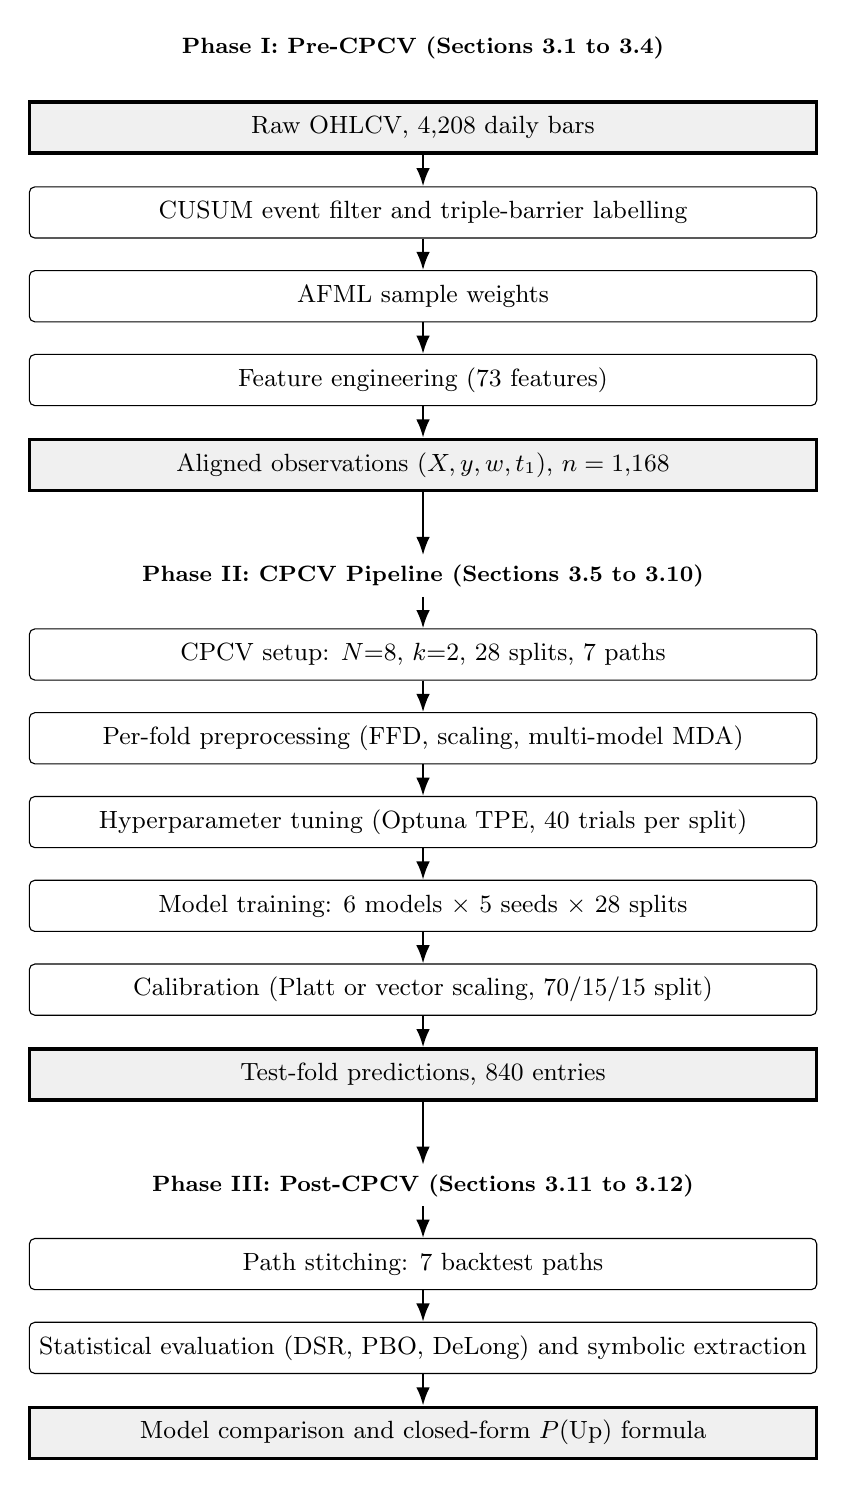
\begin{tikzpicture}[
    node distance=4mm,
    every node/.style={font=\small},
    process/.style={rectangle, draw, rounded corners=2pt, minimum width=10cm, minimum height=0.65cm, align=center},
    data/.style={rectangle, draw, very thick, minimum width=10cm, minimum height=0.65cm, align=center, fill=gray!12},
    phase/.style={font=\footnotesize\bfseries, align=center, minimum width=10cm},
    arrow/.style={-Latex, thick}
]

\node[phase] (p1) {Phase I: Pre-CPCV (Sections 3.1 to 3.4)};
\node[data, below=of p1] (a) {Raw OHLCV, 4,208 daily bars};
\node[process, below=of a] (b) {CUSUM event filter and triple-barrier labelling};
\node[process, below=of b] (c) {AFML sample weights};
\node[process, below=of c] (d) {Feature engineering (73 features)};
\node[data, below=of d] (e) {Aligned observations $(X, y, w, t_1)$, $n = 1{,}168$};

\node[phase, below=8mm of e] (p2) {Phase II: CPCV Pipeline (Sections 3.5 to 3.10)};
\node[process, below=of p2] (f) {CPCV setup: $N{=}8$, $k{=}2$, 28 splits, 7 paths};
\node[process, below=of f] (g) {Per-fold preprocessing (FFD, scaling, multi-model MDA)};
\node[process, below=of g] (h) {Hyperparameter tuning (Optuna TPE, 40 trials per split)};
\node[process, below=of h] (i) {Model training: 6 models $\times$ 5 seeds $\times$ 28 splits};
\node[process, below=of i] (j) {Calibration (Platt or vector scaling, 70/15/15 split)};
\node[data, below=of j] (k) {Test-fold predictions, 840 entries};

\node[phase, below=8mm of k] (p3) {Phase III: Post-CPCV (Sections 3.11 to 3.12)};
\node[process, below=of p3] (l) {Path stitching: 7 backtest paths};
\node[process, below=of l] (m) {Statistical evaluation (DSR, PBO, DeLong) and symbolic extraction};
\node[data, below=of m] (n) {Model comparison and closed-form $P(\textup{Up})$ formula};

\foreach \src/\dst in {a/b, b/c, c/d, d/e, e/p2, p2/f, f/g, g/h, h/i, i/j, j/k, k/p3, p3/l, l/m, m/n} {
    \draw[arrow] (\src) -- (\dst);
}

\end{tikzpicture}
\caption{End-to-end methodology pipeline. Light-bordered boxes are processing steps, dark-bordered shaded boxes are data states. \hyperref[ref:pipeline_call]{$\hookleftarrow$}}
\label{fig:pipeline_diagram}
\end{figure}

\subsection{Labelling Diagnostics}\label{app:labelling_diagnostics}

\begin{figure}[H]
\centering
\includegraphics[width=\textwidth]{ewma_vol.png}
\caption{EWMA daily volatility of BTC-USD log returns with span 50, annualised by $\sqrt{365}$. \hyperref[ref:ewma_call]{$\hookleftarrow$}}
\label{fig:ewma_vol}
\end{figure}

\begin{figure}[H]
\centering
\includegraphics[width=\textwidth]{cusum_filter_example.png}
\caption{CUSUM event filter applied to BTC daily log returns over a three-month window. \hyperref[ref:cusum_call]{$\hookleftarrow$}}
\label{fig:cusum_window}
\end{figure}

\begin{figure}[H]
\centering
\includegraphics[width=0.7\textwidth]{label_distribution.png}
\caption{Class distribution of the 1,168 binary-labelled observations after rare-class removal. \hyperref[ref:label_dist_call]{$\hookleftarrow$}}
\label{fig:label_distribution}
\end{figure}

\subsection{Weighting Diagnostics}\label{app:weighting_diagnostics}

\begin{figure}[H]
\centering
\includegraphics[width=\textwidth]{sample_weights.png}
\caption{Sample weight diagnostics. Left: distribution of per-event weights after the AFML four-step scheme and 99th-percentile capping. Right: weights over time. \hyperref[ref:weights_call]{$\hookleftarrow$}}
\label{fig:sample_weights}
\end{figure}

\begin{table}[H]
\centering
\begin{tabular}{lrrrr}
\toprule
Date & Weight & Label & Return & Holding (days) \\
\midrule
2018-11-14 & 2.862 & $-1$ & $-0.151$ & 5 \\
2019-03-29 & 2.862 & $+1$ & $+0.191$ & 4 \\
2020-03-08 & 2.862 & $-1$ & $-0.387$ & 4 \\
2021-02-03 & 2.862 & $+1$ & $+0.233$ & 5 \\
2022-09-06 & 2.862 & $+1$ & $+0.135$ & 3 \\
2022-11-04 & 2.862 & $-1$ & $-0.123$ & 4 \\
2023-02-09 & 2.862 & $+1$ & $+0.114$ & 6 \\
2023-03-13 & 2.862 & $+1$ & $+0.133$ & 4 \\
2023-10-20 & 2.862 & $+1$ & $+0.115$ & 3 \\
2025-02-26 & 2.862 & $+1$ & $+0.117$ & 4 \\
2025-10-05 & 2.862 & $-1$ & $-0.083$ & 5 \\
2026-02-03 & 2.862 & $-1$ & $-0.171$ & 2 \\
\bottomrule
\end{tabular}
\caption{Events at or above the 99th-percentile weight cap (2.862). \hyperref[ref:weights_call]{$\hookleftarrow$}}
\label{tab:capped_events}
\end{table}


\subsection{Full Feature List}\label{app:features}

\begin{longtable}{p{3.5cm}p{7cm}p{2.5cm}}
\caption{Full feature list (73 features) grouped by family. \hyperref[ref:features_call]{$\hookleftarrow$}}
\label{tab:full_features} \\

\toprule
Feature & Description & Parameters \\
\midrule
\endfirsthead

\multicolumn{3}{c}{\tablename\ \thetable{} -- continued from previous page} \\
\toprule
Feature & Description & Parameters \\
\midrule
\endhead

\midrule
\multicolumn{3}{r}{\textit{Continued on next page}} \\
\endfoot

\bottomrule
\endlastfoot

\multicolumn{3}{l}{\textbf{Technical Analysis (25), from BTC OHLCV}} \\
\midrule
Daily log returns & Log of close-to-close return & --- \\
Realised volatility & Rolling standard deviation of log returns, annualised by $\sqrt{365}$ & 21-day window \\
Garman-Klass volatility & Range-based volatility using OHLC \citep{garman_klass_1980} & 21-day window \\
Yang-Zhang volatility & Range-based volatility with overnight correction \citep{yang_zhang_2000} & 21-day window \\
ATR (log) & Average True Range, EWMA-smoothed, log-transformed & span 14 \\
Bollinger Band width & $(upper - lower) / middle$ on closing price & 20-day, $2\sigma$ \\
Volatility term 7/30 & 7-day over 30-day realised volatility ratio & 7d / 30d \\
Volatility term 30/90 & 30-day over 90-day realised volatility ratio & 30d / 90d \\
RSI & Relative Strength Index with Wilder smoothing & 14-day \\
MACD line & $EMA(12) - EMA(26)$ of close & 12, 26 \\
MACD signal & $EMA(9)$ of MACD line & 9 \\
MACD histogram & MACD line minus MACD signal & derived \\
ROC 14 & 14-day rate of change of close & 14-day \\
Stochastic \%K & Stochastic oscillator on close & 14-day \\
Stochastic \%D & 3-period SMA of \%K & 3 \\
Williams \%R & Williams percent-range oscillator & 14-day \\
CCI & Commodity Channel Index & 14-day \\
OBV (log) & On-Balance Volume, sign-preserving log transform & cumulative \\
Chaikin oscillator & $EMA(3) - EMA(10)$ of accumulation/distribution line & 3, 10 \\
MFI & Money Flow Index & 14-day \\
Rolling skewness & Rolling skewness of daily log returns & 21-day window \\
Rolling kurtosis & Rolling kurtosis of daily log returns & 21-day window \\
EMA ratio 20/50 & 20-day EMA over 50-day EMA & 20 / 50 \\
EMA ratio 50/200 & 50-day EMA over 200-day EMA & 50 / 200 \\
VWMA ratio 20/50 & 20-day volume-weighted MA over 50-day VWMA & 20 / 50 \\

\midrule
\multicolumn{3}{l}{\textbf{Mathematical (9), from BTC log returns and log prices (AFML Part 4)}} \\
\midrule
Shannon entropy & Rolling entropy of discretised log returns & 30-day window \\
Lempel-Ziv complexity & Compressibility of binarised return sequence & 90-day window \\
Negentropy & Gap between Gaussian maximum-entropy and empirical entropy & 30-day window \\
Hurst exponent & Rescaled-range analysis with sub-windows 14, 30, 60, 90 days & 180-day window \\
Variance ratio & Lo-MacKinlay variance-ratio test \citep{lo_mackinlay_1988} & 90-day, lag 7 \\
Jarque-Bera & Joint test of skewness and excess kurtosis & 90-day window \\
SADF & Supremum Augmented Dickey-Fuller statistic & min sub-length 90, lag 1 \\
SMT polynomial-1 & Sub/Super-Martingale Test with degree-1 polynomial trend & rolling \\
SMT exponential & Sub/Super-Martingale Test with exponential trend & rolling \\

\midrule
\multicolumn{3}{l}{\textbf{External: Macro (20), from Yahoo Finance and FRED}} \\
\midrule
DXY ROC 30 & 30-day rate of change of US Dollar Index & 30-day \\
US 2Y yield & 2-year US Treasury yield (FRED DGS2, T10Y2Y fallback) & level \\
US 10Y yield & 10-year US Treasury yield (Yahoo \textasciicircum TNX) & level \\
2Y-10Y slope & 10Y yield minus 2Y yield & level \\
10Y-30Y slope & 30Y yield minus 10Y yield & level \\
VIX & CBOE Volatility Index & level \\
S\&P 500 ret 30 & 30-day return of S\&P 500 index & 30-day \\
S\&P 500 ret 14 & 14-day return of S\&P 500 index & 14-day \\
Nasdaq ret 30 & 30-day return of Nasdaq Composite & 30-day \\
Nasdaq ret 14 & 14-day return of Nasdaq Composite & 14-day \\
Gold ret 30 & 30-day return of gold spot & 30-day \\
Gold ret 14 & 14-day return of gold spot & 14-day \\
Silver ret 30 & 30-day return of silver spot & 30-day \\
Silver ret 14 & 14-day return of silver spot & 14-day \\
Copper ret 30 & 30-day return of copper futures & 30-day \\
Copper ret 14 & 14-day return of copper futures & 14-day \\
Oil ret 30 & 30-day return of WTI crude oil & 30-day \\
Oil ret 14 & 14-day return of WTI crude oil & 14-day \\
Natgas ret 30 & 30-day return of natural gas & 30-day \\
Natgas ret 14 & 14-day return of natural gas & 14-day \\

\midrule
\multicolumn{3}{l}{\textbf{External: Crypto cross-sectional (1), from CoinMetrics with Yahoo Finance fallback}} \\
\midrule
ETH/BTC ratio & Daily ETH-USD over BTC-USD price ratio & level \\

\midrule
\multicolumn{3}{l}{\textbf{External: On-chain (8), from CoinMetrics, shifted by one trading day}} \\
\midrule
Active addresses ROC 14 & 14-day rate of change of daily active addresses & 14-day \\
Tx count ROC 14 & 14-day rate of change of transaction count & 14-day \\
Hash rate ROC 30 & 30-day rate of change of network hash rate & 30-day \\
MVRV & Market-Value-to-Realised-Value ratio & level \\
Net exchange flow & Net daily flow of coins to or from exchanges & level \\
Fee per tx & Average daily fee per transaction & level \\
Exchange supply \% & Fraction of supply held on exchange-attributed addresses & level \\
Issuance & Daily native-unit issuance of newly mined coins & level \\

\midrule
\multicolumn{3}{l}{\textbf{Lag (10), from BTC log returns}} \\
\midrule
Log returns lag 1 & 1-day lag of daily log returns & 1-day \\
Log returns lag 2 & 2-day lag of daily log returns & 2-day \\
Log returns lag 3 & 3-day lag of daily log returns & 3-day \\
Log returns lag 4 & 4-day lag of daily log returns & 4-day \\
Log returns lag 5 & 5-day lag of daily log returns & 5-day \\
Log returns lag 6 & 6-day lag of daily log returns & 6-day \\
Log returns lag 7 & 7-day lag of daily log returns & 7-day \\
Log returns lag 14 & 14-day lag of daily log returns & 14-day \\
Log returns lag 21 & 21-day lag of daily log returns & 21-day \\
Log returns lag 30 & 30-day lag of daily log returns & 30-day \\

\end{longtable}

\subsection{CPCV Split Details}\label{app:cpcv_splits}

\begin{figure}[H]
\centering
\includegraphics[width=\textwidth]{cpcv_groups.png}
\caption{Eight CPCV groups overlaid on BTC closing price, each holding 146 of the 1,168 aligned observations. \hyperref[ref:cpcv_groups_call]{$\hookleftarrow$}}
\label{fig:cpcv_groups}
\end{figure}

\begin{table}[H]
\centering
\begin{tabular}{lcrrcc}
\toprule
Split & Test groups & Train & Test & Leaks & Status \\
\midrule
0 & (0, 1) & 865 & 292 & 0 & OK \\
1 & (0, 2) & 851 & 292 & 0 & OK \\
2 & (0, 3) & 853 & 292 & 0 & OK \\
3 & (0, 4) & 853 & 292 & 0 & OK \\
4 & (0, 5) & 853 & 292 & 0 & OK \\
5 & (0, 6) & 853 & 292 & 0 & OK \\
6 & (0, 7) & 864 & 292 & 0 & OK \\
7 & (1, 2) & 864 & 292 & 0 & OK \\
8 & (1, 3) & 852 & 292 & 0 & OK \\
9 & (1, 4) & 852 & 292 & 0 & OK \\
10 & (1, 5) & 852 & 292 & 0 & OK \\
11 & (1, 6) & 852 & 292 & 0 & OK \\
12 & (1, 7) & 863 & 292 & 0 & OK \\
13 & (2, 3) & 862 & 292 & 0 & OK \\
14 & (2, 4) & 850 & 292 & 0 & OK \\
15 & (2, 5) & 850 & 292 & 0 & OK \\
16 & (2, 6) & 850 & 292 & 0 & OK \\
17 & (2, 7) & 861 & 292 & 0 & OK \\
18 & (3, 4) & 864 & 292 & 0 & OK \\
19 & (3, 5) & 852 & 292 & 0 & OK \\
20 & (3, 6) & 852 & 292 & 0 & OK \\
21 & (3, 7) & 863 & 292 & 0 & OK \\
22 & (4, 5) & 864 & 292 & 0 & OK \\
23 & (4, 6) & 852 & 292 & 0 & OK \\
24 & (4, 7) & 863 & 292 & 0 & OK \\
25 & (5, 6) & 864 & 292 & 0 & OK \\
26 & (5, 7) & 863 & 292 & 0 & OK \\
27 & (6, 7) & 875 & 292 & 0 & OK \\
\bottomrule
\end{tabular}
\caption{Per-split leakage audit across the 28 CPCV splits. \hyperref[ref:leakage_audit_call]{$\hookleftarrow$} }
\label{tab:leakage_audit}
\end{table}

% Group boundaries, train/test timelines for all 28 splits, leakage
% audit.

\subsection{Hyperparameter Search Spaces}\label{app:hyperparams}
% Optuna search spaces for all tuned models.

\begin{table}[H]
\centering
\footnotesize
\begin{tabular}{p{1.5cm}p{1.7cm}p{2.3cm}p{5.0cm}p{2.0cm}}
\toprule
Model & Family & Architecture & Hyperparameters & Role \\
\midrule
AR Logistic & Econometric & LR on lags 1 to 7, 14, 21, 30 & $\bullet$\ deterministic: $C=1.0$, L2, balanced, max\_iter=1000 & Pure momentum baseline (Q1, Q2) \\
Logistic Regression & Linear ML & LR on MDA-selected features &
$\bullet$\ $C \in [10^{-4}, 10^{2}]$ \newline
$\bullet$\ penalty $\in \{\text{L1}, \text{L2}\}$ \newline
(balanced, max\_iter=1000)
& Linear baseline (Q3) \\
Random Forest & Ensemble & 500 trees, balanced\_subsample &
$\bullet$\ n\_estimators $\in [100, 250]$ \newline
$\bullet$\ max\_depth $\in [2, 6]$ \newline
$\bullet$\ min\_samples\_leaf $\in [15, 40]$ \newline
$\bullet$\ max\_features $\in \{\text{sqrt}, \text{log2}\}$ \newline
(n\_jobs=$-1$)
& Nonlinear ensemble (Q3) \\
XGBoost & Ensemble & 500 trees, early stopping at 20 rounds &
$\bullet$\ max\_depth $\in [1, 3]$ \newline
$\bullet$\ lr $\in [10^{-2}, 0.3]$ \newline
$\bullet$\ min\_child\_weight $\in [5, 30]$ \newline
$\bullet$\ subsample, colsample\_bytree $\in [0.6, 1.0]$ \newline
$\bullet$\ gamma $\in [10^{-8}, 1]$ \newline
$\bullet$\ reg\_alpha, reg\_lambda $\in [10^{-8}, 10]$ \newline
(binary:logistic, scale\_pos\_weight)
& Gradient boosting (Q3) \\
LSTM & Neural & window=14, single layer, last-hidden pooling &
$\bullet$\ hidden $\in \{16, 32\}$ \newline
$\bullet$\ dropout $\in [0.1, 0.5]$ \newline
$\bullet$\ lr $\in [10^{-4}, 5 \times 10^{-2}]$ \newline
($T_0=25$, batch=64, label smoothing 0.1)
& Temporal dependencies (Q3) \\
KAN & Neural & efficient\_kan $[n, \text{width}_1, 2]$, single hidden, spline order 3 &
$\bullet$\ width$_1 \in [2, 6]$ \newline
$\bullet$\ grid $\in \{3, 5\}$ \newline
$\bullet$\ lr $\in [5 \times 10^{-4}, 5 \times 10^{-2}]$ \newline
$\bullet$\ weight\_decay $\in [10^{-5}, 5 \times 10^{-3}]$ \newline
(width$_2=0$, $T_0=30$, label smoothing 0.1)
& Interpretable architecture (Q3, Q4) \\
\bottomrule
\end{tabular}
\caption{Summary of the six models. Tuned hyperparameter ranges are listed as bullets, with fixed parameters in parentheses. \hyperref[ref:model_summary_call]{$\hookleftarrow$}}
\label{tab:model_summary}
\end{table}


\subsection{Mathematical Supplements}\label{app:math}

\subsubsection{Fractional-difference weight recursion}\label{app:ffd_weights}
The weights $\{\omega_k\}_{k \geq 0}$ for the fractional difference of order $d$ follow the recursion
\[
\omega_0 = 1, \qquad \omega_k = -\omega_{k-1} \cdot \frac{d - k + 1}{k}.
\]
The weight series is truncated at the first $k$ for which $|\omega_k| < 10^{-4}$, or at $k = 200$, whichever comes first, to keep the convolution finite. Referenced from Section 3.6.1. \hyperref[ref:ffd_weights_call]{$\hookleftarrow$}


\subsubsection{Deflated Sharpe Ratio}\label{app:dsr_formula}
The Deflated Sharpe Ratio of \citet[Chapter 11]{lopez_de_prado_2018} is
\[
\text{DSR} = \Phi\!\left(\frac{\text{SR}_{\text{observed}} - E[\max \text{SR}]}{\sigma_{\text{SR}}}\right),
\]
with the expected maximum Sharpe across $n$ candidate strategies
\[
E[\max \text{SR}] = \sqrt{2 \ln n}\left(1 - \frac{\gamma}{2 \ln n}\right) + \frac{\gamma}{2\sqrt{2 \ln n}},
\]
and the Sharpe standard error
\[
\sigma_{\text{SR}} = \sqrt{\frac{1 - \text{skew} \cdot \text{SR} + \tfrac{\text{kurt} + 2}{4} \cdot \text{SR}^2}{n_{\text{obs}} - 1}},
\]
where $\gamma$ is the Euler-Mascheroni constant. For normal returns ($\text{skew} = 0$, raw $\text{kurt} = 3$) the standard error reduces to $\sqrt{(1 + \text{SR}^2 / 2) / (n_{\text{obs}} - 1)}$. Referenced from Section 3.10.3. \hyperref[ref:dsr_formula_call]{$\hookleftarrow$}


\subsubsection{DeLong pairwise AUC test}\label{app:delong_formula}
For the pairwise AUC comparison between models $a$ and $b$, the DeLong $z$-statistic \citep{delong_1988} is
\[
z = \frac{\text{AUC}_a - \text{AUC}_b}{\sqrt{\text{Var}(\text{AUC}_a) + \text{Var}(\text{AUC}_b) - 2 \, \text{Cov}(\text{AUC}_a, \text{AUC}_b)}},
\]
where $\text{Var}$ and $\text{Cov}$ are computed by the structural-component method on the pooled predicted probabilities. The two-sided $p$-value is obtained from the standard normal CDF. Referenced from Section 3.10.3. \hyperref[ref:delong_formula_call]{$\hookleftarrow$}


\subsection{Symbolic Extraction Pipeline Details}\label{app:symbolic_details}

This appendix collects the per-step parameters, the candidate library, the known fragilities, and the workarounds for the symbolic-extraction pipeline of Section 3.11. The main-text section carries the high-level pipeline description and the load-bearing design decisions, with everything here held out of the main text for compactness. \hyperref[ref:symbolic_appendix_call]{$\hookleftarrow$}


\subsubsection{Fold selection and data preparation}\label{app:symbolic_fold_setup}

The locked-run configuration selects split 27 (the last split) on the rationale given in Section 3.11. An alternative rule of selecting the fold with the highest KAN F1 was considered but rejected, since it would bias selection toward the best-performing fold and trade away the deployment-scenario interpretation. After fold selection, the stored $d^{\ast}$ from Section 3.6.1 is applied to the full ATR series before extracting the training-fold values, and the stored RobustScaler is applied to the training-fold features. The input dimensionality is reduced to the top three features by 28-fold MDA selection frequency, with the choice of three trading input signal against the readability of the resulting closed-form expression. The selected features are chronologically partitioned 80/20 into a model-training portion and a validation portion, with a tanh input normalisation $z = \tanh((x - \mu) / (\sigma + 10^{-8}))$ fitted on the model-training portion and applied unchanged to the validation portion to keep input values bounded in $[-1, 1]$. The locked-run output is a training set of 540 events and a validation set of 135 events. The PyKAN architecture uses module-level defaults of hidden width 5, grid size 5, and spline order 3, with a data-aware safety floor that requires at least 5 training samples per model parameter.


\subsubsection{Four-step PyKAN algorithm: full parameter detail}\label{app:symbolic_algorithm}

Step 1 is a three-phase training schedule. Phase 1 runs 600 Adam steps at learning rate $10^{-3}$ and weight decay $10^{-3}$, with Gaussian noise injection at standard deviation 0.05 clamped to $[-1, 1]$ acting as a dropout-like regulariser, and early stopping driven by validation loss. Phase 2a runs 20 LBFGS steps at learning rate $10^{-2}$ with no regularisation. Phase 2b runs another 20 LBFGS steps at the same learning rate with combined L1 and entropy regularisation at $\lambda = 0.002$, which encourages the sparse activations the pruning step will exploit. Grid extension is disabled throughout because with 540 training samples a grid refinement from 3 to 5 would add parameters faster than the data can support. A dynamic majority-baseline gate after Phase 1 and a structurally similar gate at the pre-prune stage check the validation accuracy against $\max(0.53, \text{val\_majority\_baseline} + 0.01)$ and log a warning if the model has not learned beyond the baseline.

Step 2 prunes the trained model. A forward pass on the validation set populates cached activations, and a call to PyKAN's \textit{attribute} method scores each edge by activation magnitude. Edges with importance below the threshold 0.01 are removed by \textit{prune}, with a multi-API fallback because the method signature varies across PyKAN versions. The pruned model is verified to still produce a valid forward pass, and the operation reverts to the pre-prune state if any edge removal breaks the topology.

Step 3 replaces each surviving spline edge with the best-fitting symbolic function from a library of 14 candidates: the polynomials $x$, $x^2$, $x^3$, $x^4$, the transcendentals $\exp$, $\log$, $\sqrt{\cdot}$, $\tanh$, $\sin$, $\cos$, $\arctan$, the non-smooth primitives $|x|$ and $\text{sgn}(x)$, and the zero function. For each edge $(l, i, j)$, the call \textit{suggest\_symbolic} returns the top five candidates ranked by goodness of fit, and the per-edge winner is the candidate with the highest $R^2$ above 0.30. Below threshold, the edge keeps its spline form. The zero function is a special case because PyKAN's candidate-ranking loss penalises complexity in addition to fit error, so the zero function wins on the combined loss regardless of fit quality. A brute-force fallback iterates manually through the other 13 candidates whenever \textit{suggest\_symbolic} returns zero, capturing per-candidate $R^2$ from PyKAN's stdout via regex and selecting the best non-constant function with $R^2 \geq 0.30$.

Step 4 fine-tunes the affine parameters of each symbolic edge. Each edge has the form $a \cdot f(b x + c) + d$ for a chosen function $f$, and the four scalars are updated by 30 LBFGS steps at learning rate $4 \times 10^{-4}$. A NaN check after each LBFGS step reverts the model to its pre-fine-tune state if the update produces a non-finite parameter.


\subsubsection{Formula extraction and known fragilities}\label{app:symbolic_fragilities}

After the four steps complete, the model produces two output expressions, $\text{logit}_{\text{bearish}}$ for class 0 and $\text{logit}_{\text{bullish}}$ for class 1. SymPy simplifies the decision function $\text{logit}_{\text{bullish}} - \text{logit}_{\text{bearish}}$ into a closed-form expression in the surviving features, with a 30-second timeout that prevents the simplification routine from hanging on pathological inputs. The surviving features are those that appear in the free symbols of the simplified decision function, which is generally a subset of the three input features since pruning may remove all edges associated with a feature.

Two PyKAN behaviours have downstream methodological consequences. First, the absolute-value primitive $|x|$ symbolises cleanly through \textit{fix\_symbolic} but produces a SymPy expression that is non-differentiable at zero. For features whose mean falls close to zero in the tanh-normalised space, the partial-derivative sensitivity analysis of Chapter 4 returns NaN at the mean, which is discussed as L6 in Section 5.4. Second, the brute-force fallback for symbolification parses PyKAN's standard output via a regular expression to recover per-candidate $R^2$ values. The fallback works on the PyKAN version pinned in this thesis but is fragile to library upgrades, since the stdout format is not part of PyKAN's public API.


\subsection{Per-Split Classification Reports}\label{app:split_reports}
% 28 splits x 6 models.

\subsection{Symbolic Extraction Detailed Output}\label{app:symbolic}
% Full PyKAN training logs, edge-by-edge R^2, pruned diagrams,
% unsimplified formulas.

\subsection{Leakage Prevention Summary}\label{app:leakage_summary}
% T-R15 / T-R17 (write for reviewers; easy to teach). Moved to the
% appendix during the page-budget pass; lives here as a single-page
% reference for defenders and reviewers who want a per-channel audit.
%
% Table suggestion: leakage prevention summary
%   Risk                                  | Mitigation                                                           | Where
%   FFD d* on full data                   | per-fold training-only estimation                                    | preprocessing.py
%   Scaler on full data                   | RobustScaler on training fold only                                   | preprocessing.py
%   Feature selection on full data        | multi-model MDA on training fold only                                | preprocessing.py
%   HP tuning on full data                | nested Optuna inside training fold (3-fold purged)                   | tuning.py
%   Overlapping TBL labels                | three-condition purging                                              | cv.py
%   Serial correlation across CV boundary | embargo after test boundary                                          | cv.py
%   Calibration on test data              | held-out 15\% calibration partition of training fold, never test     | calibration.py
%   XGB early-stop + cal shared cell      | acknowledged; only ensemble size affected                            | pipeline.py
%   On-chain look-ahead                   | CoinMetrics shifted by 1 day                                         | external\_features.py
%   CUSUM threshold on full data          | minor approximation; acknowledged, negligible impact                 | labeling.py
%   NaN imputation across train-test      | ffill().bfill() independent within each partition; FFD columns drop  | preprocessing.py


% =============================================
% End Document
% =============================================
\end{document}
